\chapter{Gäste- und Themenstruktur}

Nachdem die untersuchten Sendungen charakterisiert und in die Geschichte der Talkshow eingeordnet wurde, soll sich nun der Präsentation der Untersuchungsergebnisse zugewendet werden. Im ersten Teil der Ergebnispräsentation stehen die quantitativen Auswertungen im Mittelpunkt. Die Auswertung erfolgte dabei in Hinblick auf zwei Ziele. Erstens soll dargestellt werden ob und inwieweit die Polittalks den Kriterien der Vielfalt und Relevanz entsprechen und zweitens geht es darum Unterschieden bzw. Gemeinsamkeiten zwischen den einzelnen Sendungen herauszuarbeiten.

\section{Themenstruktur}

Zuerst wird die Themenstruktur der untersuchten Talkshows dargestellt, im zweiten Unterkapitel folgt dann die Gästestruktur.

\subsection{Themenbereiche}\label{chap:themenbereiche}

Wenig überraschend dominieren bei allen Sendungen politische und wirtschaftliche Themen. Insgesamt sind 65 \% aller untersuchten Talkfolgen in diesen beiden Themenbereichen zu verorten, wobei Wirtschaftsthemen hiervon allerdings nur 20,8 \% ausmachen. An dritter Stelle folgen Gesundheitsthemen mit 10,2 \%. Wie Abbildung \vref{plot:themenverteilung} zu entnehmen ist, gibt es bei der gesamten ARD-Talkschiene eine ähnliche Verteilung. Unterschiede zeigen sich in einem etwas geringeren Anteil von Wirtschaftsthemen und dem etwas höheren Anteil des Personality- und Prominenzbereich, bedingt durch die beiden ARD-Talks \textit{Beckmann} und \textit{Menschen bei Maischberger}.

Zwischen den einzelnen Sendungen gibt es allerdings große Unterschiede. \textit{Günther Jauch} setzt fast ausschließlich auf politische (65 \%) beziehungsweise wirtschaftliche Themen (20 \%). Gleiches gilt für \textit{Anne Will}, auch dort beträgt der Anteil an Wirtschafts- und Politikthemen über 80 \%. Ein etwas anderes Bild ergibt sich für \textit{maybrit illner}. Dort wurde fast gleich stark auf Wirtschafts- (41,5 \%) und Politikthemen (48,8 \%) gesetzt. Dieser hohe Wirtschaftsanteil ist im Vergleich zu den anderen Talks auffällig, da dort nur in zwischen 27 \% und 9,8 \% der Fälle solche Themen diskutiert wurden. Der Unterschied erklärt sich fast ausschließlich durch die häufige Thematisierung der Eurokrise bei \textit{maybrit illner}. Die drei erwähnten Sendungen lassen sich hinsichtlich ihrer Themenbereiche somit als klassische Polittalks charakterisieren. Damit einhergeht im Falle von \textit{Günther Jauch} und \textit{maybrit illner} ein begrenzter Themenmix – nur fünf der neun Themenbereiche werden abgedeckt.

\begin{figure}[ht]
	%Do not try to scale figure in .tex or you loose font size consistency
	\centering
	%The code to input the plot is extremely simple
	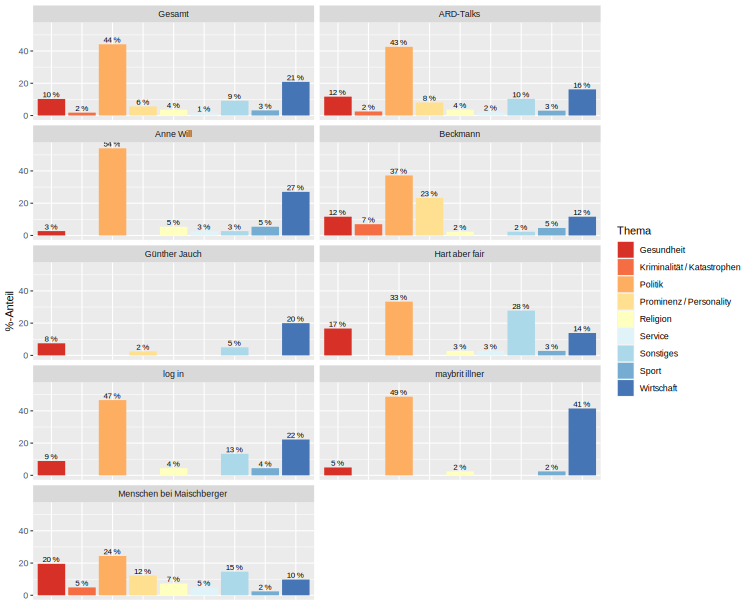
\includegraphics[width=1\textwidth]{daten/grafiken/plot_themenverteilung.png}
	%Captions and Labels can be used since this is a figure environment
	\caption{Themenverteilung innerhalb der Sendungen}
	\subcaption*{vgl. auch ausführliche Tabelle \vref{tab:anhang_themenbereiche_sendungen} im Anhang}
	\label{plot:themenverteilung}
\end{figure}

Wie Abbildung \vref{plot:themenverteilung} zeigt, gibt es dahingegen bei \textit{Beckmann} und \textit{Menschen bei Maischberger} mit ihren relativ geringen Anteilen an politischen und wirtschaftlichen Themen den breitesten Themenmix. Dies zeigt die Nähe der beiden Sendungen zum Personality-Talk und betont zugleich, dass sie thematisch nicht eindeutig dem Polittalk zugeschlagen werden können. Insbesondere \textit{Menschen bei Maischberger} kommt bloß auf einen Politikanteil von 24,4 \%.

Hinsichtlich \textit{hart aber fair} ist der geringe Politik- (33,3 \%) und Wirtschaftsanteil (13,9 \%) und der gleichzeitig relativ breite Themenmix hingegen überraschend, beschreibt sich die Sendung selbst doch als harter Politiktalk. Tatsächlich setzte \textit{hart aber fair} im Untersuchungszeitraum jedoch relativ stark auf Gesundheitsthemen sowie auf Themen, die sich nicht eindeutig einer Kategorie zuordnen ließen. Schaut man sich diese Folgen genauer an, so stellt man fest, dass es sich vor allem um ethische und moralische Fragen handelt. Aber auch exotische Themen werden behandelt, so trug die \textit{hart aber fair} Folge vom 23. April 2012 beispielsweise den Titel „Wissen wo der Hammer hängt – was treibt die Deutschen in den Baumarkt?“.

\textit{log in} unterscheidet sich bei der Themenwahl auf dieser Ebene nicht stark von den anderen Talks. Dies war aber auch nicht unbedingt zu erwarten, schließlich hat die Sendung ebenfalls den Anspruch ein Polittalk zu sein.

Die sieben Sendungen lassen sich anhand der behandelten Themenbereiche in zwei Gruppen einteilen, die sich untereinander nur wenig unterscheiden. In der einen Gruppe finden sich die Sendungen mit relativ hohem Politik- und Wirtschaftsanteil – \textit{Anne Will}, \textit{Günther Jauch} sowie \textit{log in} und maybrit illner. Die zweite Gruppe besteht hingegen aus den Sendungen die einen breiteren Themenmix anbieten – \textit{Beckmann}, \textit{hart aber fair} und \textit{Menschen bei Maischberger}. Wirklich klare Themenprofile, die einer Sendung ein absolutes Alleinstellungsmerkmal geben würden, lassen sich auf dieser Untersuchungsebene nicht feststellen.

\subsubsection{Politikbereiche}

Hinsichtlich der thematisierten Politikbereiche lässt sich festhalten, dass innenpolitische Themen in allen Sendungen klar dominieren (vgl. Abbildung \vref{plot:politikbereiche}), am stärksten bei \textit{Beckmann}, wo fast keine anderen Politikbereiche behandelt werden. \textit{Günther Jauch}, \textit{log in} und \textit{maybrit illner} folgen mit jeweils circa 60 \% Innenpolitikanteil. Einzig \textit{Menschen bei Maischberger} hat genauso oft sozialpolitische wie innenpolitische Themen im Programm. Allerdings ist hier, wie bereits erwähnt, der Anteil politischer Sendungen bereits von vornherein sehr gering. Ähnlich stellt sich die Situation bei hart aber fair dar, hier liegt das Verhältnis von innen- zu sozialpolitischen Themen bei 42 \% zu 33 \%. Einen relativ hohen Anteil an Themen aus dem Bereich der Sozialpolitik hat ebenfalls noch Anne Will (35 \%), allerdings nicht zu Lasten der Innenpolitik, sondern aller anderen Politikbereiche.

Während sich sozialpolitische Thematiken zumindest in allen untersuchten Sendungen fanden, kamen Themen aus dem Bereich der Bildungspolitik gerade einmal in einer Talkshow vor, nämlich in der \textit{Günther Jauch} Folge vom 27. November 2011 mit dem Titel „Generation doof – warum gibt es so viele Bildungsverlierer?“. \textit{Günther Jauch} ist zudem die einzige Sendung, die alle der sechs erfassten Politikbereiche abdeckt. \textit{Beckmann} dagegen behandelt nur innen- und sozialpolitische Themen.

Ebenfalls vernachlässigt werden die Themenbereiche Außen- und Umwelt- bzw. Energiepolitik. \textit{maybrit illner} und \textit{Günther Jauch} kommen immerhin auf zwei Folgen zu außenpolitischen Themen innerhalb eines Jahres und haben damit absolut gesehen den Spitzenplatz inne. Dies ist erstaunlich, hätte es doch innerhalb des Untersuchungszeitraums mehr als genug relevante Anlässe für eine Talkrunde gegeben – man denke nur an die Ereignisse in Ägypten, Tunesien und Libyen im Zuge des sogenannten Arabischen Frühlings.

\begin{figure}[ht]
	%Do not try to scale figure in .tex or you loose font size consistency
	\centering
	%The code to input the plot is extremely simple	
	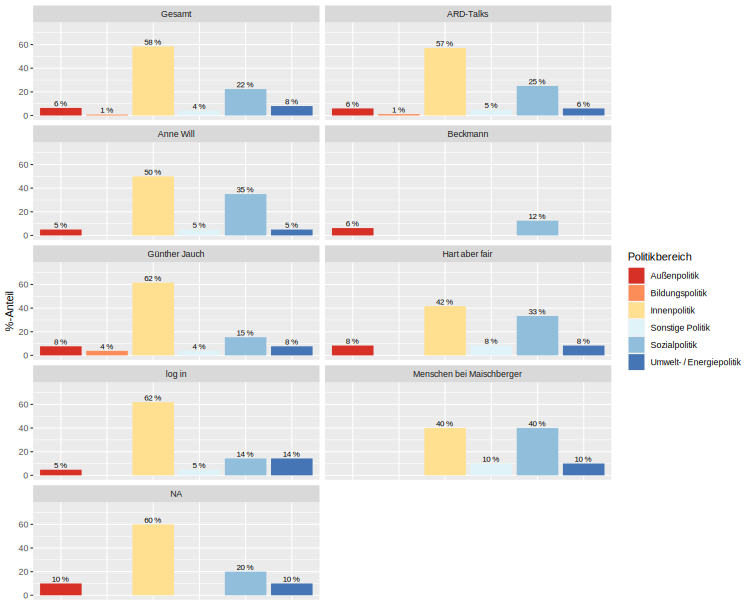
\includegraphics[width=1\textwidth]{daten/grafiken/plot_politikbereiche.png}
	%Captions and Labels can be used since this is a figure environment
	\caption{Politikbereiche nach Sendungen}
	\label{plot:politikbereiche}
	\subcaption*{vgl. auch ausführliche Tabelle \vref{tab:anhang_politikbereiche_sendungen} im Anhang}
\end{figure}

Gleiches gilt für die Umwelt- und Energiepolitik, einzig log in kümmerte sich intensiver um dieses Thema und widmete ihm immerhin drei seiner 21 Talks zu politischen Themen. Damit kann sich die Sendung ein wenig von den anderen untersuchten Talks abheben.

Ergebnisse früherer Untersuchungen werden somit bestätigen \parencite[8f.]{muellerSchaubuehneFuerEinflussreichen2006}: Die Innenpolitik ist sehr dominant, daneben finden eigentlich nur noch sozialpolitischen Themen größere Beachtung in den Sendungen. Alle anderen hier erfassten Politikbereiche – Außen-, Umwelt- bzw. Energiepolitik sowie Bildungspolitik – finden sich hingegen nur selten in den Polittalks. Aus Perspektive der zuvor erläuterten Qualitätskriterien ist dies natürlich problematisch, werden doch hier durchaus wichtige Politikbereiche – etwa die Außenpolitik – stiefmütterlich behandelt und sich fast ausschließlich auf innenpolitische Themen konzentriert. Diese Einseitigkeit setzt sich bei der Themenwahl fort, wie der folgende Abschnitt darlegt.

\subsection{Themencluster}\label{chap:themencluster}

Während die Einteilung in Themenbereiche ein grobes Raster ist, das zwar größere Tendenzen aufzeigen kann – etwa das Vernachlässigen außenpolitischer Fragen – zeigt doch erst eine Einteilung in Themencluster, inwiefern sich Themen tatsächlich wiederholen.

Die häufigsten Themen sind die Eurokrise, mit großem Abstand gefolgt von der sogenannten Wulff-Affäre und dem recht umfassenden Thema Ernährung sowie der Wahl des neuen Bundespräsidenten Joachim Gauck und den beiden sozialpolitischen Themen Renten und soziale Gerechtigkeit – und zwar sowohl im gesamten Sample als auch bei der ARD-Talkschiene alleine (vgl. Tabelle \vref{tab:themencluster}).

\begin{table}[ht]
	\centering
	\caption{Häufige Themencluster}
	\resizebox{\textwidth}{!}{%
		\begin{tabular}{@{}lcccc@{}}
			\toprule
			\multicolumn{1}{c}{\textbf{Themencluster}} & \textbf{Alle Sendungen} & \textbf{Anteil (n=283)} & \textbf{ARD-Talks} & \textbf{Anteil (n=197)} \\ \midrule
			Eurokrise & 47 & 16,6\% & 24 & 12,2\% \\
			Wulff-Affäre & 23 & 8,1\% & 17 & 8,6\% \\
			Ernährung & 11 & 3,9\% & 9 & 4,6\% \\
			Bundespräsident Gauck & 9 & 3,2\% & 7 & 3,6\% \\
			Renten & 8 & 2,8\% & 5 & 2,5\% \\
			Soziale Gerechtigkeit & 8 & 2,8\% & 7 & 3,6\% \\ \bottomrule
		\end{tabular}
	}
	\label{tab:themencluster}
\end{table}

Der Dauerbrenner ist sowohl bei den beiden ZDF-Talks als auch in der ARD-Talkschiene die Eurokrise. In 53 Kalenderwochen des Untersuchungszeitraums wurde mindestens eine der untersuchten Polittalks gesendet. Angesichts von 47 Talkfolgen zur Eurokrise muss man also festhalten, dass dieses Thema theoretisch fast jede Woche Gegenstand der Sendungen war. Nun mag die Eurokrise zwar ein hochdynamisches, komplexes Thema sein, bei dem ein hoher Diskussionsbedarf auch in der Bevölkerung besteht – eine derart häufige Behandlung scheint aber doch übertrieben, dürften hier doch zahlreiche Wiederholungen unvermeidlich sein.

Um herauszufinden, ob es zudem zeitlich begrenzte Themenballungen gab, wurden die Häufigkeit der Themen nach Monaten aufgeschlüsselt. Bei den meisten Themen findet sich eine relativ ausgewogene Verteilung, bei bestimmten spektakulären und kontroversen Themen fanden sich hingegen auffällige Häufungen.

\subsubsection{Die Wulff-Affäre}

Ein solches ist die sogenannte Wulff-Affäre, die sich ab Anfang Dezember 2011 entfaltete und im Rücktritt des damaligen Bundespräsidenten Christian Wulff am 17. Februar 2012 gipfelte. Im Zeitraum vom 14. Dezember 2011 bis zum 11. März 2012 widmen die untersuchten Polittalks diesem Thema allein 23 ihrer Folgen und damit gut 34 \% der in diesem Zeitraum ausgestrahlten Folgen.
Zeitweise fand in den Talks kaum ein anderes Thema statt. In der Woche vom 8. bis zum 12. Januar 2012 hatten beispielsweise fünf der sieben untersuchten Sendungen Wulff zum Thema (vgl. Tabelle \vref{tab:wulff-talks1}).

\begin{table}[ht]
	\centering
	\caption{Talks zur Wulff-Affäre zwischen dem 8. und 12. Januar 2012}
	\resizebox{\textwidth}{!}{%
		\begin{tabular}{@{}lll@{}}
			\toprule
			\multicolumn{1}{c}{\textbf{Datum}} & \multicolumn{1}{c}{\textbf{Sendung}} & \multicolumn{1}{c}{\textbf{Titel}}                                                  \\ \midrule
			8. Januar 2012                     & Günther Jauch                        & Der Problem-Präsident – wie glaubwürdig ist Christian Wulff                         \\
			9. Januar 2012                     & hart aber fair                       & Der Pattex-Präsident – was lehrt der Fall Wulff?                                    \\
			11. Januar 2012                    & log in                               & Liebling, ich habe das Amt geschrumpft - Brauchen wir noch einen Bundespräsidenten? \\
			12. Januar 2012                    & Beckmann                             & Macht, Medien, Moral – wo sind Deutschlands Vorbilder?                              \\
			12. Januar 2012                    & maybrit illner                       & Affäre Wulff: Vorhang zu und viele Fragen offen?                                    \\ \bottomrule
		\end{tabular}
	}
	\label{tab:wulff-talks1}
\end{table}

Als Anfang März die Diskussion über Wulffs Ehrensold aufkam, nahmen das nochmals vier Sendungen zum Anlass innerhalb weniger Tage diesem Thema eine Diskussion zu widmen (vgl. Tabelle \vref{tab:wulff-talks2}).

\begin{table}[ht]
	\centering
	\caption{Talks zur Wulff-Affäre zwischen dem 6. und 11. März 2012}
	\resizebox{\textwidth}{!}{%
		\begin{tabular}{@{}lll@{}}
			\toprule
			\multicolumn{1}{c}{\textbf{Datum}} & \multicolumn{1}{c}{\textbf{Sendung}} & \multicolumn{1}{c}{\textbf{Titel}}                                     \\ \midrule
			6. März 2012                       & Maischberger                         & Ehrensold für Wulff, Millionen für Chefs – und was kriegt der Rest?    \\
			7. März 2012                       & Anne Will                            & Mein Auto, mein Büro, mein Zapfenstreich – Was hat Wulff verdient?     \\
			8. März 2012                       & Beckmann                             & Nach dem Zapfenstreich für Wulff                                       \\
			8. März 2012                       & maybrit illner                       & Versagt, doch gut versorgt? - Wulffs Abschied mit Pauken und Moneten   \\
			11. März 2012                      & Günther Jauch                        & Der tiefe Fall des Christian Wulff – wie gelingt ein Abschied in Würde \\ \bottomrule
		\end{tabular}
	}
	\label{tab:wulff-talks2}
\end{table}

\subsubsection{Bundespräsident Gauck}

Im März 2012 ließ ich eine weitere Themenhäufung feststellen. Innerhalb von  sechs Tagen befassten sich alleine fünf Sendungen mit der (bevorstehenden) Wahl des neuen Bundespräsidenten Joachim Gauck und kaprizierten sich dabei fast ausschließlich auf eine Charakterisierung Gaucks (vgl. Tabelle \vref{tab:gauck-talks}). Eine Häufung die auch dem ARD-Programmbeirat negativ auffiel \parencite[2]{ard-programmbeiratTalkformateImErsten2012}.

\begin{table}[ht]
	\centering
	\caption{Talks zur Bundespräsidentenwahl zwischen 14. und 19. März 2012}
	\resizebox{\textwidth}{!}{%
		\begin{tabular}{@{}lll@{}}
			\toprule
			\multicolumn{1}{c}{\textbf{Datum}} & \multicolumn{1}{c}{\textbf{Sendung}} & \multicolumn{1}{c}{\textbf{Titel}}                                        \\
			\midrule
			14. März 2012                      & Anne Will                            & Bundespräsident Gauck – bekommen wir endlich den Richtigen?               \\
			15. März 2012                      & Beckmann                             & Die Präsidentenmacher – Drei Tage vor der Wahl des neuen Staatsoberhaupts \\
			15. März 2012                      & maybrit illner                       & Gauck for President - fast alle für einen, einer für alle?                \\
			18. März 2012                      & Günther Jauch                        & Joachim Gauck – der Volks-Präsident                                       \\
			19. März 2012                      & hart aber fair                       & Der Bewährungshelfer – kann Gauck das Ansehen der Politiker heilen?       \\
			\bottomrule
		\end{tabular}
	}
	\label{tab:gauck-talks}
\end{table}

Derartige Themenballungen lassen sich immer wieder – wenn auch meist in kleinerem Umfang – im Beobachtungszeitraum finden. Zum Beispiel beschäftigten sich innerhalb von fünf Wochen zwei Talks mit dem Thema Burnout – wobei in diesem Fall nicht zu erwarten ist, dass sich innerhalb dieser Zeit neue Erkenntnis ergeben haben.

Bei einigen Themen wird man dies zwar dadurch rechtfertigen können, dass das Thema aus einem anderen Blickwinkel beleuchtet wird, die Sendungen stark unterschiedliche Zielgruppen ansprechen oder das Thema eine solche Relevanz besitzt, dass eine mehrmalige Thematisierung lohnt. Häufungen wie zuvor exemplarisch dargestellt, wenn sich also innerhalb eines kurzen Zeitraums fast alle Sendungen dem gleichen Thema widmen, lassen sich so allerdings nicht rechtfertigen. Hier ist schlicht und ergreifend ermüdende Wiederholung des immer gleichen an der Tagesordnung, während andere – eventuell genauso relevante Themen – nicht behandelt werden und damit auch von einer pluralen Themensetzung keine Rede mehr sein kann.

\subsection{Titelgebung}\label{chap:titelgebung}

Nicht systematisch untersucht wurde die Titelgebung der einzelnen Talkshowfolgen. Ein Blick auf den Korpus macht dennoch deutlich, dass viele Titel Formulierungen benutzen, die einen Skandal oder eine drohende Katastrophe suggerieren und damit Angst wecken bzw. zumindest provokativ wirken.

Meist wird dem Titel ein Fragezeichen nachgestellt, um so den Eindruck einer ergebnisoffenen Diskussion zu erwecken was allerdings meist schon durch den Rest des Titels konterkariert wird. Besonders deutlich wird dies, wenn man die Titel mit denen älterer Sendungen vergleicht. \textcite[195f.]{kellerGeschichteTalkshowDeutschland2009} gibt einige Titel aus den 1960er Jahren wieder, diese zeichnen sich meist durch neutrale und einfache Frageformulierungen aus – etwa: „Lässt sich Bildung planen?“\footnote{Zugegebenermaßen finden sich solche Titel bereits in der großen politischen Talkshow der 90er Jahre, Talk im Turm, seltener \parencite[301f.]{kellerGeschichteTalkshowDeutschland2009}.}. Heutige Titel versuchen dagegen durch Emotionalisierung die Zuschauer anzusprechen, dramatisieren damit aber von vornherein die Themen und schränken die Diskussion zudem durch Vorfestlegungen bereits im Vorhinein ein.

Tabelle \vref{tab:talktitel} dokumentiert eine kleine Auswahl an exemplarischen Titeln, die obigen Befund veranschaulichen:

\begin{table}[ht]
	\centering
	\caption{Ausgewählte Titelbeispiele}
	\resizebox{\textwidth}{!}{%
		\begin{tabular}{@{}lll@{}}
			\toprule
			\multicolumn{1}{c}{\textbf{Datum}} & \multicolumn{1}{c}{\textbf{Sendung}} & \multicolumn{1}{c}{\textbf{Titel}}                                                \\ \midrule
			  25. April 2012 & Anne Will & Preis-Wahnsinn an der Zapfsäule – Autofahren bald unbezahlbar? \\
			  24. November 2011& Beckmann & Krankenhaus-Keime – Die unsichtbare Gefahr \\
			  9. Oktober 2011& Günther Jauch & Essen für die Tonne – wie stoppen wir den Wegwerf-Wahnsinn? \\
			  16. Juli 2012& hart aber fair& Umsorgt vom Kreißsaal bis zum Hörsaal – kommt jetzt die Generation Weichei? \\
			  29. Februar 2012 & log in& Teuro-Sprit und Turbo-Protzer – Sind Autos von gestern? \\
			  6. Oktober 2012& maybrit illner& Burnout – muss bald ganz Deutschland auf die Couch?\\
			  27. September 2011 & Maischberger & Machofrauen – Müde Männer: Letzte Runde im Geschlechterkampf? \\ \bottomrule
		\end{tabular}
	}
\label{tab:talktitel}
\end{table}

\section{Gästestruktur}

Nachdem die Themenstruktur bereits gewisse Einseitigkeiten und Unzulänglichkeiten offenbart hat, wird im Weiteren die Gästestruktur der gleichen Analyse unterzogen.

\subsection{Personenspektrum}\label{chap:personenspektrum}

Bei der Untersuchung der Gästestruktur ist zuvorderst die Frage interessant, ob die  Talkshows – wie ihnen regelmäßig vorgeworfen wird – immer wieder die gleichen Personen einladen. Ob also eine Art „Talkelite“ besteht und diese somit bevorzugt ihre Interessen und Meinungen den Zuschauern präsentieren können\footnote{Natürlich lassen sich aufgrund der Ergebnisse nur bedingt Aussagen zum Prozess der Gästeauswahl treffen. So ist es prinzipiell möglich, dass die verschiedenen Redaktionen sich durchaus bemühen ein plurales Gästespektrum sicher zu stellen, ihre Bemühungen aber aufgrund von Absagen und ähnlichem scheitern.}.

\subsubsection{Alle Sendungen}

Insgesamt waren in allen erfassten Sendungen 1441 Gäste eingeladen. Etwas mehr als die Hälfte davon nur einmal (753), zweimal waren 120 Personen eingeladen, dreimal  44 und viermal 23. Fünf- bzw. sechsmal waren noch 15 bzw. 10 Personen eingeladen.

Die Gästeliste wird angeführt von elf Personen, die zwischen sieben und elfmal an einer politischen Talkshow teilnahmen. Zusammen bestreiten diese Personen etwa zehn Prozent der Auftritte. Die Spitzenposition hat dabei CDU-Arbeits- und Sozialministerin Ursula von der Leyen inne. Von den elf Personen sind wiederum acht Politiker (vgl. Tabelle \vref{tab:gaesterangliste}). Wir werden später noch sehen, dass oftmals die gleichen Politiker eingeladen werden. Die Bedeutung der Werte wird klar, wenn man sich vor Augen führt, dass innerhalb des Untersuchungszeitraums in 53 Wochen Polittalks ausgestrahlt wurden, das heißt, dass beispielsweise Ursula von der Leyen rein statistisch in elf dieser 53 Wochen als Gast in einer der sieben Talkshows zugegen war. Dies wären immerhin etwa 30 \% des Untersuchungszeitraums.

\begin{table}[ht]
	\centering
	\caption{Gästerangliste}
%	\resizebox{\textwidth}{!}{%
		\begin{tabular}{@{}llll@{}}
			\toprule
			\multicolumn{1}{c}{\textbf{Gast}} & \multicolumn{1}{c}{\textbf{Rolle}} & \multicolumn{1}{c}{\textbf{Auftritte}} & \multicolumn{1}{c}{\textbf{Anteil}} \\ \midrule
			Ursula von der Leyen              & Politiker                          & 11                                     & 0,76\%                              \\
			Wolfgang Bosbach                  & Politiker                          & 10                                     & 0,69\%                              \\
			Dirk Müller                       & Finanzexperte                      & 9                                      & 0,62\%                              \\ 
			Peter Altmaier                    & Politiker                          & 9                                      & 0,62\%                              \\
			Sahra Wagenknecht                 & Politikerin                        & 9                                      & 0,62\%                              \\
			Hans-Ulrich Jörges                & Journalist                         & 8                                      & 0,56\%                              \\
			Christian Lindner                 & Politiker                          & 7                                      & 0,49\%                              \\
			Gertrud Höhler                    & Publizistin                        & 7                                      & 0,49\%                              \\
			Gregor Gysi                       & Politiker                          & 7                                      & 0,49\%                              \\
			Jürgen Trittin                    & Politiker                          & 7                                      & 0,49\%                              \\
			Wolfgang Kubicki                  & Politiker                          & 7                                      & 0,49\%                              \\
			10 Gäste                          &                                    & 6                                      & 4,16\%                              \\
			15 Gäste                          &                                    & 5                                      & 5,20\%                              \\
			23 Gäste                          &                                    & 4                                      & 6,38\%                              \\
			44 Gäste                          &                                    & 3                                      & 9,16\%                              \\
			120 Gäste                         &                                    & 2                                      & 16,52\%                             \\
			751 Gäste                         &                                    & 1                                      & 52,26\%                             \\
			\midrule
			&                                    &                                        & 100,00\% \\
			\bottomrule                           
		\end{tabular}
%	}
	\subcaption*{alle Sendungen; n=1441}
	\label{tab:gaesterangliste}
\end{table}

\subsubsection{Die Sendungen im Vergleich}

Betrachtet man die Sendungen getrennt voneinander, so ergibt sich ein differenzierteres Bild. Um aussagekräftigere und leichter vergleichbare Ergebnisse zu erzielen, wurde ein Wiederholungsquotient errechnet. Hierzu wurde die Anzahl an Gästen durch die Anzahl an individuellen Personen dividiert. Hierdurch erhält man eine Zahl zwischen 1 und x. Wenn der Quotient 1 ist heißt das, dass die Zahl der Auftritte mit der Zahl individueller Personen identisch ist, mithin jeder Talkgast bloß einmal eingeladen war. Ist das Ergebnis hingegen zwei, so bedeutet dies, dass im Durchschnitt jede Person zweimal zu Gast war.
 
\begin{figure}[ht]
	%Do not try to scale figure in .tex or you loose font size consistency
	\centering
	%The code to input the plot is extremely simple
	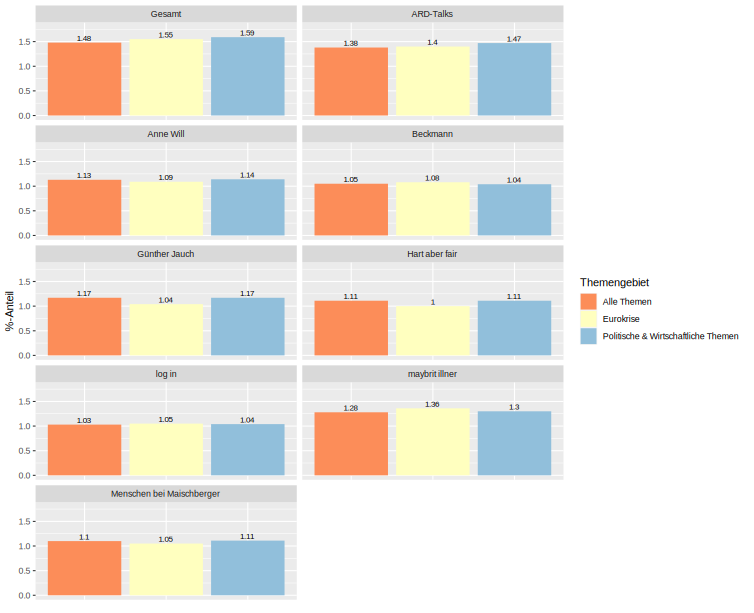
\includegraphics[width=1\textwidth]{daten/grafiken/plot_wdhquote_gaeste.png}
	%Captions and Labels can be used since this is a figure environment
	\caption{Wiederholungsquotient (alle Gäste)}
	\label{plot:whdquote_gaeste}
\end{figure}

Wie bei Betrachtung von Abbildung \vref{plot:whdquote_gaeste} deutlich wird, gibt es zwischen den einzelnen Sendungen teils deutliche Unterschiede. Während bei \textit{log in} und \textit{Beckmann} nur äußerst selten Gäste mehrfach auftauchen, findet sich bei \textit{maybrit illner} ein relativ hoher Quotient von 1,28 – sprich es traten innerhalb der Sendung häufiger Personen mehrfach auf als in den anderen Polittalks.

Dennoch sind die Quotienten innerhalb der Sendungen gering im Vergleich zu denen zwischen den Sendungen. Sowohl innerhalb der ARD-Talkschiene als auch zwischen allen untersuchten Polittalks kommt es zu häufigeren Gästewiederholungen. Dies spricht dafür, dass die einzelnen Redaktionen zwar darauf achten, dass innerhalb ihrer Sendung nicht allzu oft die gleichen Personen auftreten, dies aber zwischen den Sendungen nicht gelingt.

Besonders auffällig ist, dass der Wiederholungsquotient bei politischen und wirtschaftlichen Themen bei fast allen Sendungen höher ist als im Gesamtschnitt. Über alle Sendungen hinweg beträgt der Quotient hier fast 1,6, was darauf hindeutet, dass es bei politischen und wirtschaftlichen Themen tatsächlich eine Art Talkelite gibt, die zwar nicht unbedingt immer wieder in der gleichen Sendung zu Gast ist, dafür stattdessen durch alle Sendungen tingelt.

Ähnliches gilt hinsichtlich der Wiederholungsquote bei Talks zur Eurokrise. Auch dort liegt der Quotient bei den einzelnen Sendungen meist relativ niedrig, oftmals sogar niedriger als im Gesamtschnitt. Über alle Sendungen hinweg hingegen ist die Wiederholungsquote mit 1,55 dagegen fast genauso hoch wie bei den politischen und wirtschaftlichen Themen.

\subsubsection{Politische Talkelite – Talkende Politikerelite}

Das obige Ergebnis wird noch verstärkt, wenn die Gäste nach ihren Funktionen getrennt betrachtet werden. Hier wird erneut bestätigt, dass es eine Art Politikelite gibt, die immer wieder eingeladen wird. So treten zwar in den untersuchten Sendungen 424-mal Politiker auf, diese Auftritte werden aber nur von 196 unterschiedlichen Personen bestritten (vgl. Tabelle \vref{tab:poltikerauftritte}).

\begin{table}[ht]
	\centering
	\caption{Auftritte von Politikern}
	\resizebox{\textwidth}{!}{%
		\begin{tabular}{@{}lll@{}}
			\toprule
			\multicolumn{1}{c}{\textbf{Gäste}} & \multicolumn{1}{c}{\textbf{Anzahl an Auftritte}} & \multicolumn{1}{c}{\textbf{\%-Anteil an den Auftritten}} \\ \midrule
			Ursula von der Leyen & 11 & 2,6\%   \\
			Wolfgang Bosbach & 10  & 2,4\%   \\
			2 Politiker & Je 9 & 4,3\%   \\
			4 Politiker & Je 7 & 6,6\%   \\
			6 Politiker & Je 6 & 8,5\%   \\
			8 Politiker & Je 5 & 9,4\%   \\
			13 Politiker & Je 4 & 12,3\%  \\
			15 Politiker & Je 3 & 10,6\%  \\
			38 Politiker & Je 2 & 17,9\%  \\
			108 Politiker & Je 1 & 25,5\%  \\ \midrule
			Insgesamt 196 & Insgesamt 424 & 100,0\% \\ \bottomrule
		\end{tabular}
	}
	\label{tab:poltikerauftritte}
\end{table}

Dies ergibt einen Wiederholungsquotienten von 2,16 und bedeutet das im Durchschnitt jeder Politiker mehr als zweimal in den Polittalks auftrat. Bei Journalisten beträgt der Wert nur noch 1,56, bei Experten und Wirtschaftsvertretern noch 1,35 bzw. 1,34. Vertreter von Religionsgemeinschaften und Normalbürger sind fast ausschließlich nur einmal Gast in den untersuchten Sendungen (vgl. Abbildung \vref{plot:whdquote_gaeste_allg}). Die Beschränkung auf wenige Personen mit häufigem Erscheinen ist also nicht bei allen Gästegruppen gleich stark ausgeprägt.

\begin{figure}[ht]
	%Do not try to scale figure in .tex or you loose font size consistency
	\centering
	%The code to input the plot is extremely simple
	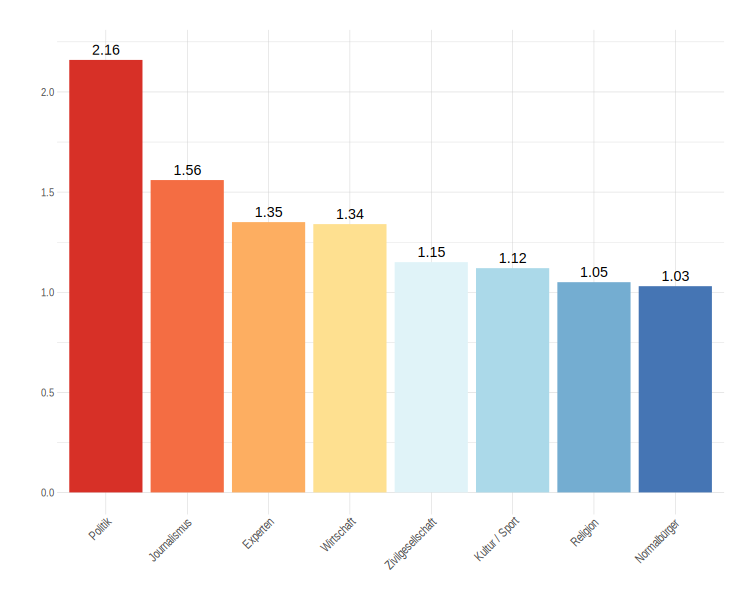
\includegraphics[width=1\textwidth]{daten/grafiken/plot_wdhquote_gaeste_allg.png}
	%Captions and Labels can be used since this is a figure environment
	\caption{Wiederholungsquotient (Auftritte / Personen) nach Rollen}
	\label{plot:whdquote_gaeste_allg}
\end{figure}

\subsubsection{Talkelite in der Eurokrise}

Doch findet sich dieses Bild bei allen Themen? Ein Blick auf die Situation beim Thema Eurokrise bestätigt dies nicht. Zwar liegt auch hier der Wiederholungsquotient bei Politikern am höchsten, gleichzeitig ist er aber zum einen um 0,46 Punkte niedriger und zum anderen liegt er insbesondere bei Experten und Vertretern aus dem Bereich Wirtschaft nun deutlich höher (vgl. Abbildung \vref{plot:whdquote_gaeste_euro}).

Die Vermutung liegt nahe, dass es also je nach Thema unterschiedliche Talkeliten gibt. Eine entsprechende Analyse kann an dieser Stelle leider nicht für jedes Thema erfolgen, da dies den Rahmen sprengen würde. Bei Talks zur Eurokrise jedenfalls findet sich statt einer reinen Politikerelite, vielmehr eine Gästeelite aus Experten und Personen aus den Bereichen Politik und Wirtschaft.

\begin{figure}[ht]
	%Do not try to scale figure in .tex or you loose font size consistency
	\centering
	%The code to input the plot is extremely simple
	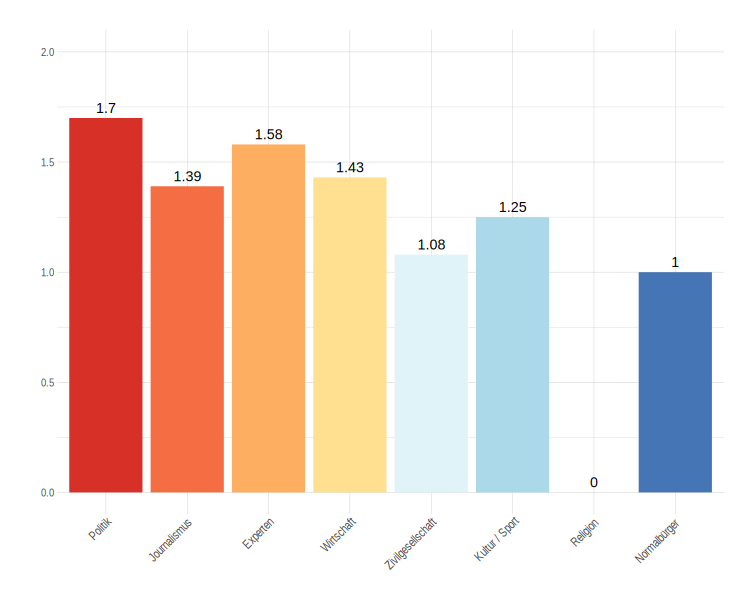
\includegraphics[width=1\textwidth]{daten/grafiken/plot_wdhquote_gaeste_euro.png}
	%Captions and Labels can be used since this is a figure environment
	\caption{Wiederholungsquotient (Auftritte / Personen) nach Rollen (Eurokrise)}
	\label{plot:whdquote_gaeste_euro}
\end{figure}

\subsection{Gesellschaftliche Rollen}\label{chap:gesellschaftlicherollen}

Bei der Analyse politischer Talkshows sind nicht nur einzelne Personen und die Häufigkeit ihres Auftretens interessant, sondern auch welche gesellschaftlichen Rollen diese Personen vertreten und ob sich hier eventuell ebenfalls Einseitigkeiten feststellen lassen\footnote{Da Personen durchaus mehrere gesellschaftliche Rollen inne haben können, erfolgte die Zuordnung zu den Kategorien jeweils auf Basis der Vorstellung der jeweiligen Gäste in den Sendungen bzw. auf der zugehörigen Internetseite. Dies ist insofern sinnvoll, als man davon ausgehen kann, dass die jeweiligen Personen aufgrund dieser gesellschaftlichen Rolle in die Sendung eingeladen wurden.}.

\subsubsection{Gesamtbild}

Die in Tabelle \vref{tab:prozent-rollen} aufgeführte prozentuale Rollenverteilung zeigt, dass insgesamt Politiker am häufigsten eingeladen waren, also genau die Gruppe deren individuelle Vertreter oft mehrmals eingeladen wurden (vgl. Kapitel \vref{chap:personenspektrum}). Mit über zehn Prozentpunkten Abstand folgen dicht beieinander Personen aus dem kulturellen und sportlichen Bereich, Experten und Journalisten. Knapp dahinter liegen Wirtschaftsvertreter mit circa zehn Prozent. Weit seltener zu Gast waren wiederum „Normalbürger“, Vertreter der Zivilgesellschaft – also von Vereinen, Verbänden oder Non Governmental Organisations (NGOs) – und von Religionsgemeinschaften.

Ähnlich stellt sich die Verteilung dar, wenn nur die Sendungen der ARD-Talkschiene betrachtet werden. Zwar werden etwas häufiger Personen aus dem Bereich Journalismus, Kultur / Sport, sowie Experten und „Normalbürger“ eingeladen und etwas seltener aus  Wirtschaft, Zivilgesellschaft und Politik. Die Unterschiede bewegen sich aber im ein bis zweistelligen Prozentbereich und sind damit marginal. Dennoch kann insgesamt nicht von einer Dominanz aller Sendungen durch Politiker die Rede sein, machen sie doch insgesamt weniger als ein Drittel der Gäste aus.

\begin{table}[ht]
	\centering
	\caption{Prozentuale Rollenverteilung}
	\resizebox{\textwidth}{!}{%
		\begin{tabular}{@{}lllll@{}}
			\toprule
			&
			\multicolumn{1}{c}{\textbf{\begin{tabular}[c]{@{}c@{}}Alle Folgen\\ (n=1441)\end{tabular}}} &
			\multicolumn{1}{c}{\textbf{\begin{tabular}[c]{@{}c@{}}ARD-Talkschiene\\ (n=1044)\end{tabular}}} &
			\multicolumn{1}{c}{\textbf{\begin{tabular}[c]{@{}c@{}}Politische Themen\\ (n=640)\end{tabular}}} &
			\multicolumn{1}{c}{\textbf{\begin{tabular}[c]{@{}c@{}}Eurokrise\\ (n=229)\end{tabular}}} \\ \midrule
			\textbf{Politik}           & 29,40\%  & 26,10\%  & 39,70\%  & 44,50\%  \\
			\textbf{Kultur / Sport}    & 16,10\%  & 18,50\%  & 12,00\%  & 2,20\%   \\
			\textbf{Experten}          & 15,60\%  & 16,50\%  & 10,80\%  & 16,60\%  \\
			\textbf{Journalismus}      & 14,70\%  & 16,10\%  & 16,40\%  & 17,00\%  \\
			\textbf{Wirtschaft}        & 9,90\%   & 9,20\%   & 9,40\%   & 13,10\%  \\
			\textbf{„Normalbürger“}    & 7,40\%   & 8,60\%   & 5,30\%   & 0,90\%   \\
			\textbf{Zivilgesellschaft} & 5,30\%   & 3,40\%   & 5,60\%   & 5,70\%   \\
			\textbf{Religion}          & 1,50\%   & 1,50\%   & 0,80\%   & 0,00\%   \\
			\textbf{Sonstige}          & 0,10\%   & 0,10\%   & 0,00\%   & 0,00\%   \\
			\midrule
			\textbf{Alle Sendungen}    & 100,00\% & 100,00\% & 100,00\% & 100,00\% \\ \bottomrule
		\end{tabular}
	}
	\label{tab:prozent-rollen}
\end{table}

Bei den Talks zum Thema Eurokrise bzw. allgemein zu politischen Themen kann hingegen von einer derartigen Dominanz gesprochen werden. Dort kommen 44,5 \% respektive 39,7 \% der Gäste aus dem Politikbetrieb. Ebenfalls stärker als im Gesamtschnitt sind Personen aus der Wirtschaft anwesend. Vertreter von Religionsgemeinschaften, aus dem Bereich des kulturellen und sportlichen Lebens, sowie „Normalbürger“ sind gar nicht oder sehr selten eingeladen. Angesichts des Themas ist dies allerdings nicht verwunderlich.

Bei politischen Themen im Allgemeinen machen „Normalbürger“ hingegen immerhin 5,3 \% der Gäste aus – und damit fast genauso viele wie die Repräsentanten der Zivilgesellschaft. Etwas seltener als im Gesamtschnitt in den Runden zugegen sind Gäste aus Kultur und Sport, sowie überraschenderweise Experten, die bei der Eurokrise noch über dem Durchschnitt aller Folgen lagen.

\subsubsection{Sendungen im Vergleich}

\begin{figure}[ht]
	%Do not try to scale figure in .tex or you loose font size consistency
	\centering
	%The code to input the plot is extremely simple
	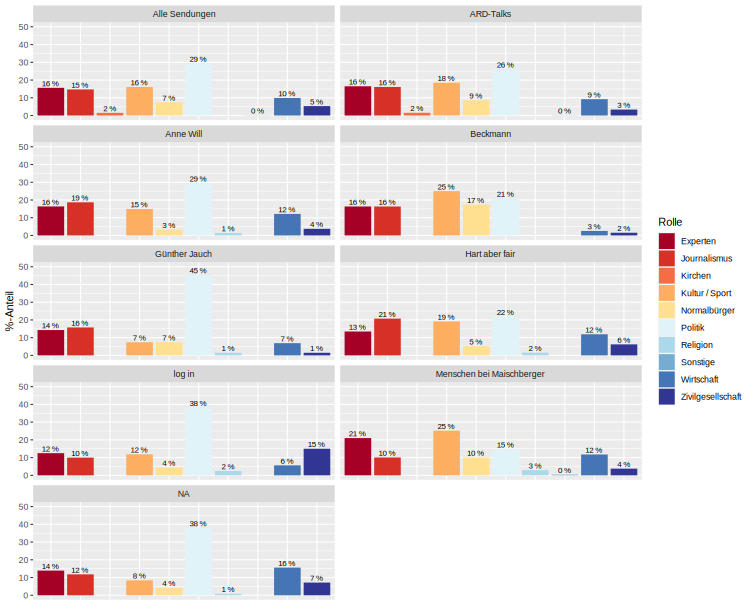
\includegraphics[width=1\textwidth]{daten/grafiken/plot_rollenverteilung.png}
	%Captions and Labels can be used since this is a figure environment
	\caption{Prozentuale Rollenverteilung (nach Sendungen getrennt)}
	\subcaption*{(vgl. auch ausführliche Tabelle \vref{tab:anhang_gaestegruppen_sendungen} im Anhang)}
	\label{plot:rollenverteilung}
\end{figure}

Differenziert man wiederum nach Sendungen so werden einige Unterschiede deutlich, die auf die unterschiedlichen Ausrichtungen der Polittalks hindeuten (vgl. Abbildung \vref{plot:rollenverteilung}). Das Flaggschiff der ARD, \textit{Günther Jauch}, gibt sich erwartungsgemäß ähnlich parteinah wie früher \textit{Sabine Christiansen} \parencite[4f.]{muellerSchaubuehneFuerEinflussreichen2006}, und erreicht einen Anteil von über 45 \% bei den Gästen aus dem politisch-administrativen Bereich. Hier kann entsprechend tatsächlich von einer Politikerdominanz der Gästestruktur gesprochen werden. Ähnlich hohe Werte erreichen noch \textit{maybrit illner} und – überraschenderweise – \textit{log in} mit je circa 38 \%. Somit unterscheidet sich das junge Format gerade nicht durch die gesellschaftlichen Rollen seiner Gäste von den etablierten politischen Talkshows. Allerdings hat die Sendung einen hohen Anteil zivilgesellschaftlicher Akteure unter den Gästen.

Bei den beiden „weicheren“ Formaten \textit{Beckmann} und \textit{Menschen bei Maischberger} sind hingegen nicht Politiker die häufigste Gästegruppe, sondern Personen aus dem kulturellen und sportlichen Leben. Zudem finden überdurchschnittlich oft „Normalbürger“ in den Sendungen Gehör. Hiermit können sich beide von den übrigen fünf Sendungen absetzen und unterstreichen nochmals ihre Nähe zum Personality-Talk.

Ebenfalls auffallend ist die Ähnlichkeit der Gästestrukturen von hart aber fair zu \textit{Maischberger} und \textit{Beckmann}. Obwohl vom Selbstverständnis her viel stärker dem klassischen Polittalk nachempfunden, ist der Anteil politischer Gäste nur unwesentlich größer als bei \textit{Beckmann}. Gäste aus dem Bereich Kultur und Sport sind zudem die dritthäufigste Gästegruppe, wir werden im zweiten Teil der Arbeit noch sehen, dass diese Einladungen nicht immer sinnvoll sind. Es zeigt sich damit bei hart aber fair das gleiche Bild, das sich bereits bei der Themenanalyse abzeichnete.

Im nächsten Schritt werden ausgewählte Gästegruppen nochmals en Detail betrachtet. Vertreter von Religionsgemeinschaften und sonstige Gäste sind kaum unter den Teilnehmern, so dass hier auf eine detaillierte Aufschlüsselung im Folgenden verzichtet wird. Gleiches gilt für „Normalbürger“ und Personen aus dem Bereich Kultur / Sport, deren Detailanalyse für die Beantwortung der behandelten Fragestellungen keinen Gewinn verspricht.

\subsubsection{Politikebenen}

Dass Politiker die größte Gästegruppe ausmachen wurde bereits festgestellt, schaut man sich nun diese Gruppe genauer an, so zeigt sich, dass es sich wiederum hauptsächlich um Personen aus der Bundespolitik handelt (vgl. Abbildung \vref{plot:politikebenen}). Von 424 Politikern sind 289 (68 \%) solche die auf der Bundesebene politische Ämter innehaben bzw. hatten. Nur 96 (23 \%) sind Landespolitiker und nochmals weit weniger sind auf EU- bzw. kommunalpolitischer Ebene aktiv, nämlich 17 (4 \%) bzw. 7 (2 \%). Ausländische Politiker treten nur viermal (1 \%) auf. Die Unterschiede zwischen den einzelnen Sendungen sind marginal, sodass auf eine differenzierte Darstellung verzichtet wird. Ebenfalls kaum in Erscheinung treten Behördenvertreter (2 \%).

\begin{figure}[ht]
	%Do not try to scale figure in .tex or you loose font size consistency
	\centering
	%The code to input the plot is extremely simple
	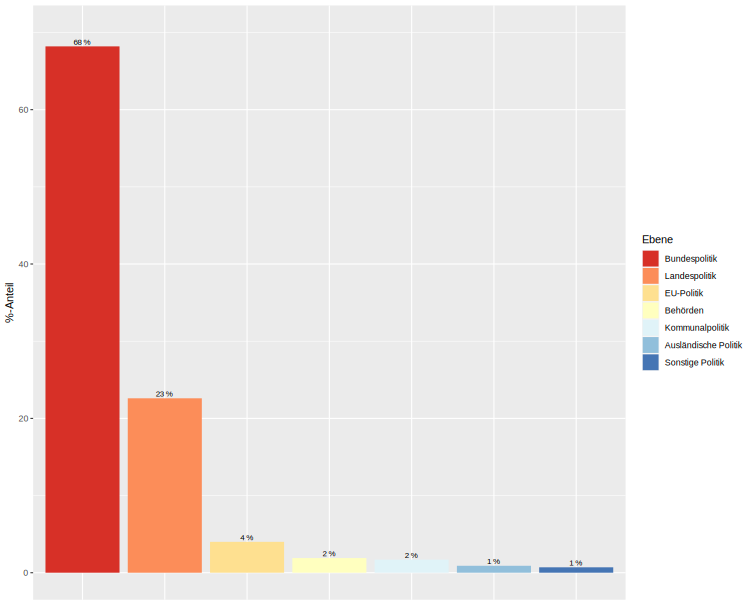
\includegraphics[width=1\textwidth]{daten/grafiken/plot_politikebenen.png}
	%Captions and Labels can be used since this is a figure environment
	\caption{Rollenverteilung innerhalb der Kategorie \textit{Politik} (n=424)}
	\label{plot:politikebenen}
\end{figure}

Dieses Übergewicht der Bundespolitik ist in mehrerlei Hinsicht problematisch. Erstens ist das hiesige politische System stark föderal geprägt, die Länder spielen im politischen Entscheidungssystem eine große Rolle, und zwar auch bei vornehmlich bundespolitischen Themen \parencite[303-331]{rudzioPolitischeSystemBundesrepublik2006}. Der geringe Anteil an Landespolitikern in den untersuchten Talkshows kann also beim Publikum ein falsches Bild über die Rolle bundespolitischer Akteure hervorrufen. Zudem gibt es zwischen den einzelnen Bundesländern Konflikte zum Beispiel über den Länderfinanzausgleich die einer öffentlichen Diskussion durchaus wert sind. Auch kommunalpolitische Themen, wie die Überschuldung der Kommunen, haben nationale Relevanz und würden eine verstärkte Einladung von Politiker aus Kommunal- und Landespolitik rechtfertigen\footnote{Zwar wurde bei der Themenanalyse nicht erfasst auf welche Politikebene sich diese beziehen, allerdings betreffen viele Themen prinzipiell auch die Bundesländer, sodass eine Unterscheidung hier per se sehr schwierig geworden wäre.}.

Zweitens tangieren Entscheidungen in Brüssel Deutschland als EU-Mitgliedsstaat. Teilweise haben dabei Entscheidungen, die von Kommission oder Europäischem Parlament getroffen werden, weitreichende Auswirkungen auf die nationale Ebene \parencite{sturmNeueDeutscheRegierungssystem2005}. Auch hier korrespondiert also nicht die Häufigkeit der Auftritte mit der tatsächlichen Wichtigkeit der Ebene im politischen Prozess. Hinzu kommt, dass der EU weiterhin die Akzeptanz in der Bevölkerung fehlt, so ist beispielsweise die Beteiligung bei den Europawahlen seit 1979 fast durchgängig gesunken \parencite{bundeszentralefuerpolitischebildungEuropawahlWahlbeteiligung197920092009}, und gleichzeitig EU-Vertreter in den Medien unterproportional häufig vorkommen \parencite{roschMedienHabenNachholbedarf2008}. Aufgabe der Polittalks wäre es in diesem Zusammenhang durch die häufigere Einladung von EU-Parlamentariern oder sonstigen Vertretern der EU diesen Effekten entgegen zu wirken, statt sie schlicht zu reproduzieren.

Ähnliches gilt für die Einladung ausländischer Politiker, die das Potenzial hätten, die Diskussion um außerdeutsche Perspektiven zu erweitern, was gerade bei der Eurokrise  sinnvoll erscheint. Doch scheuen die Redaktionen wohl den hiermit verbundenen Aufwand. so dass selbst Politiker aus den direkten Nachbarländern so gut wie nie zu Gast sind\footnote{Die ausländischen Politiker, die in den untersuchten Sendungen zu Gast waren, sind Avi Primor, der ehemalige Botschafter Israels in Deutschland, Richard Sulik, der zum damaligen Zeitpunkt Präsident des slowakischen Parlaments war und Tim Guldimann, der Schweizer Botschafter in Deutschland. Alle drei sprechen fließend deutsch und sind somit unkomplizierte Gäste.}.

Die Dominanz der Bundesebene spricht zudem dafür, dass weiterhin vor allem die politische Elite eingeladen wird \parencite[141]{doernerPolitainmentPolitikMedialen2001}.

\subsubsection{Wirtschaft}

Ebenfalls näher betrachtet werden sollen hier die Gäste aus dem wirtschaftlichen Leben, kann es doch innerhalb dieser Gruppe enorme Interessengegensätze geben. Der wichtigste ist hierbei der zwischen Kapital und Arbeit, sprich zwischen Unternehmensvertreter und Arbeitnehmer respektive ihren jeweiligen Verbänden bzw. Gewerkschaften. Von politischen Talkshows im öffentlich-rechtlichen Fernsehen wäre entsprechend zu erwarten, dass sie zumindest für ein ausgeglichenes Verhältnis zwischen beiden Seiten sorgen.

Allerdings zeigt sich ein klares Übergewicht der Arbeitgeberseite (vgl. Tabelle \vref{tab:gaeste_wirtschaft}). In sechs der sieben Sendungen waren mehr Vertreter von Unternehmen bzw. Wirtschaftsverbänden zu Gast als Gewerkschafter und Arbeitnehmer. Teilweise beträgt der Unterschied weit über 50 \%. So kommen beispielsweise in der Sendung mit dem höchsten Anteil von Gästen aus dem Bereich Wirtschaft, \textit{maybrit illner}, 62 \% mehr wirtschaftsnahe Personen zu Wort als Arbeitnehmer (-vertreter). \textit{log in} ist die einzige positive Ausnahme, der Unterschied beträgt hier nur 11,1 \% zu Lasten der arbeitnehmernahen Positionen. Allerdings kommen bei \textit{log in} insgesamt nur neun Gäste aus dem Bereich Wirtschaft vor. Noch weniger wurden nur zu \textit{Beckmann} eingeladen, dort traten fünf Vertreter von Unternehmen, zwei von Wirtschaftsverbänden und niemand von Arbeitnehmerseite auf.

Eine noch krassere Ungleichverteilung gibt es bei den Talks zur Eurokrise. Dort kommen nur bei \textit{maybrit illner} Vertreter von Arbeitnehmerseite vor und auch dann nur zwei Stück, im Gegensatz zu vierzehn von Arbeitgeberseite.

\begin{table}[ht]
	\centering
	\caption{Gäste aus dem Bereich Wirtschaft (alle Sendungen)}
	\resizebox{\textwidth}{!}{%
		\begin{tabular}{@{}ccccc@{}}
			\toprule
			&
			\textbf{Unternehmen} &
			\textbf{Wirtschaftsverband} &
			\textbf{Gewerkschaft} &
			\textbf{Arbeitnehmer} \\ \midrule
			\textbf{\begin{tabular}[c]{@{}c@{}}Anne Will\\ (n=26)\end{tabular}} &
			50,00 \% &
			23,10 \% &
			11,50 \% &
			15,40 \% \\
			\textbf{\begin{tabular}[c]{@{}c@{}}Beckmann\\ (n=5)\end{tabular}} &
			80,00 \% &
			20,00 \% &
			0,00 \% &
			0,00 \% \\
			\textbf{\begin{tabular}[c]{@{}c@{}}Günther Jauch\\ (n=14)\end{tabular}} &
			80,00 \% &
			20,00 \% &
			0,00 \% &
			0,00 \% \\
			\textbf{\begin{tabular}[c]{@{}c@{}}hart aber fair\\ (n=23)\end{tabular}} &
			43,50 \% &
			34,80 \% &
			13,00 \% &
			8,70 \% \\
			\textbf{\begin{tabular}[c]{@{}c@{}}log in\\ (n=9)\end{tabular}} &
			33,30 \% &
			22,20 \% &
			44,40 \% &
			0,00 \% \\
			\textbf{\begin{tabular}[c]{@{}c@{}}maybrit illner\\ (n=37)\end{tabular}} &
			43,20 \% &
			37,80 \% &
			16,20 \% &
			2,70 \% \\
			\textbf{\begin{tabular}[c]{@{}c@{}}Maischberger\\ (n=28)\end{tabular}} &
			57,10 \% &
			28,60 \% &
			3,60 \% &
			10,70 \% \\ \midrule
			\textbf{\begin{tabular}[c]{@{}c@{}}ARD-Talks\\ (n=96)\end{tabular}} &
			54,20 \% &
			28,10 \% &
			10,40 \% &
			7,30 \% \\
			\textbf{\begin{tabular}[c]{@{}c@{}}ARD-Talks (Eurokrise)\\ (n=13)\end{tabular}}      & 61,50 \% & 38,50 \% & 0,00 \% & 0,00 \% \\ \midrule
			\textbf{\begin{tabular}[c]{@{}c@{}}Alle Sendungen\\ (n=142)\end{tabular}} &
			50,00 \% &
			30,30 \% &
			12,00 \% &
			7,70 \% \\
			\textbf{\begin{tabular}[c]{@{}c@{}}Alle Sendungen (Eurokrise)\\ (n=30)\end{tabular}} & 43,30 \% & 50,00 \% & 6,70 \% & 0,00 \% \\ \bottomrule
		\end{tabular}%
	}
	\label{tab:gaeste_wirtschaft}
\end{table}

Zwar kann eingewendet werden, dass auch Unternehmensvertreter arbeitnehmerfreundliche Positionen vertreten oder umgekehrt Gewerkschafter sich auf Seiten der Wirtschaft schlagen können. Erfahrungsgemäß entspricht dies allerdings nicht der Regel, weshalb festzuhalten bleibt, dass es Kapitalinteressen offenbar leichter haben sich in den wichtigsten deutschen Politiktalks zu Wort zu melden.

\subsubsection{Journalist und Expert}

Experten und Journalisten, die meist entweder wegen ihrer Rolle als Experten für ein bestimmtes Thema oder ihrer pointierten Meinung eingeladen werden, machen zusammen etwas mehr als 30 \% der Gäste aus. Wobei beide Gruppen etwa zu gleichen Teilen vertreten sind (vgl. Abbildung \vref{plot:journalisten_experten}).

\begin{figure}[ht]
	%Do not try to scale figure in .tex or you loose font size consistency
	\centering
	%The code to input the plot is extremely simple
	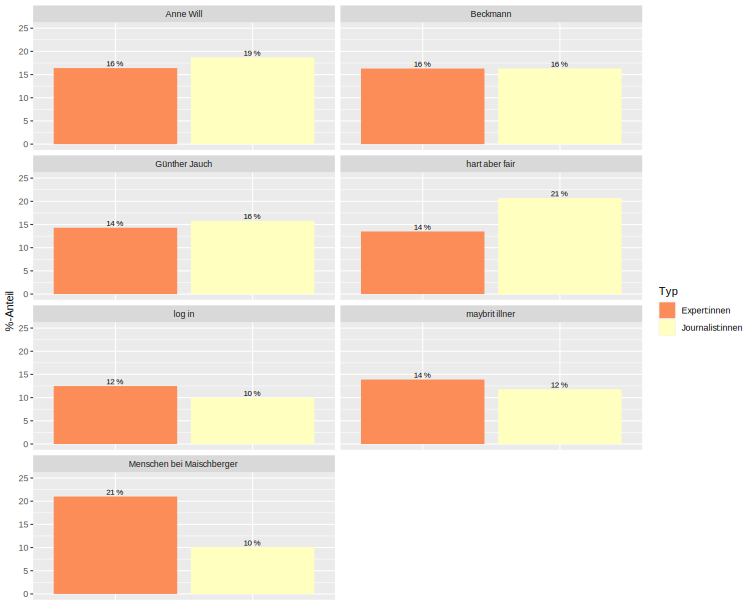
\includegraphics[width=1\textwidth]{daten/grafiken/plot_journalisten_experten.png}
	%Captions and Labels can be used since this is a figure environment
	\caption{Anteil von Journalisten und Experten nach Sendungen}
	\label{plot:journalisten_experten}
\end{figure}

In den einzelnen Sendungen ergibt sich ein ähnliches Bild wie in der Gesamtschau, allerdings zeigen sich auch hier einige Besonderheiten: Plasberg setzt stärker als alle anderen Sendungen auf die Diskussion mit seinen Berufskollegen und lädt dafür etwas weniger Experten ein. Bei Beckmann werden beide Gruppen eher selten eingeladen, genauso wie bei \textit{log in}. Hingegen setzt Maischberger stärker auf Experten, denn auf Journalisten. Es kann bei dieser Sendung also keine Rede von einem angeblich „starken Hang zur Kollegenorientierung“ \parencite{hachmeisterARDNurKeine2011} sein.

Schlüsselt man die Expertengruppe weiter auf (vgl. Tabelle \vref{tab:verteilung_experten}), so wird deutlich, dass dies bei Beckmann  und Maischberger am häufigsten Ärzte sind. Dies ist insofern logisch, als beide Sendungen relativ oft Gesundheitsthemen behandeln (vgl. Kapitel \vref{chap:themenbereiche} ). In den anderen Sendungen dominieren dagegen Wissenschaftler (\textit{Anne Will, Günther Jauch, log in, maybrit illner}). Wiederum wird daran der seriöse Anspruch der Sendungen deutlich. Einzig bei \textit{hart aber fair} stehen „sonstige Experten“ auf Platz eins, dies umfasst Politik- und Kommunikationsberater ebenso wie Personen die beispielsweise als Finanz- oder Nahostexperten vorgestellt werden ohne Hinweis auf eine eventuell universitäre oder wissenschaftliche Tätigkeit\footnote{Der Expertenstatus kann dabei durchaus zweifelhaft sein. So trat zum Beispiel allein Gertrud Höhler im Untersuchungszeitraum siebenmal auf. Vorgestellt wurde sie  meist als Politikberaterin (vgl. \textit{hart aber fair} vom 12.12.2011, \textit{Anne Will} vom 14.03. und 16.05.2012, \textit{Günther Jauch} vom 26.08.2012). Dabei gibt es allerdings erhebliche Zweifel daran, dass sie jemals als Politikberaterin tätig war \parencite{langguthLegendeKanzlerberaterin2012}. Sie selbst konnte – ironischerweise in der Talkshow \textit{Markus Lanz} – nicht erklären, wen sie beraten habe \parencite{sasseGertrudHoehlerDemontiert2012}. Den Redaktionen von \textit{Anne Will}, \textit{hart aber fair}, \textit{Günther Jauch} und \textit{Menschen bei Maischberger} kamen solche Zweifel allerdings offenbar nicht.}.

\begin{table}[ht]
	\centering
	\caption{Verteilung innerhalb der Gruppe „Experten“ (alle Sendungen)}
	\resizebox{\textwidth}{!}{%
		\begin{tabular}{@{}ccccc@{}}
			\toprule
			\textbf{} & \textbf{Wissenschaft} & \textbf{Rechtsanwälte / Juristen} & \textbf{Ärzte} & \textbf{Sonstige Experten} \\ \midrule
			\begin{tabular}[c]{@{}c@{}}Anne Will\\ (n=35)\end{tabular}       & 51,40 \% & 5,70 \%  & 20,00 \% & 22,90 \% \\
			\begin{tabular}[c]{@{}c@{}}Beckmann\\ (n=32)\end{tabular}        & 31,30 \% & 6,30 \%  & 37,50 \% & 25,00 \% \\
			\begin{tabular}[c]{@{}c@{}}Günther Jauch\\ (n=29)\end{tabular}   & 48,30 \% & 13,80 \% & 0,00 \%  & 37,90 \% \\
			\begin{tabular}[c]{@{}c@{}}hart aber fair\\ (n=26)\end{tabular}  & 30,80 \% & 11,50 \% & 15,40 \% & 42,30 \% \\
			\begin{tabular}[c]{@{}c@{}}log in\\ (n=20)\end{tabular}          & 65,00 \% & 5,00 \%  & 10,00 \% & 20,00 \% \\
			\begin{tabular}[c]{@{}c@{}}maybrit illner\\ (n=33)\end{tabular}  & 48,50 \% & 3,00 \%  & 21,20 \% & 27,30 \% \\ \midrule
			\begin{tabular}[c]{@{}c@{}}Maischberger\\ (n=50)\end{tabular}    & 28,00 \% & 4,00 \%  & 40,00 \% & 28,00 \% \\
			\begin{tabular}[c]{@{}c@{}}Alle Sendungen\\ (n=225)\end{tabular} & 41,30 \% & 6,70 \%  & 23,10 \% & 28,90 \% \\ \bottomrule
		\end{tabular}%
	}
	\label{tab:verteilung_experten}
\end{table}

\subsubsection{Zivilgesellschaft}

Vertreter der Zivilgesellschaft, also von Verbänden, Initiativen oder sozialen Bewegungen könnten ein Gegengewicht zur partei- bzw. wirtschaftsnahen Gästeauswahl bieten. Allerdings wurde bereits dargestellt, dass recht selten Gäste aus diesem Bereich eingeladen werden und ihr Anteil so insgesamt nur bei 5,3 \% liegt. Die einzige Ausnahme bildet hier \textit{log in} mit 15 \%, womit sich die Sendung von den etablierten Polittalks unterscheidet und eine größere Offenheit gegenüber außerparlamentarischen Bewegungen zeigt.

Unterteilt man die Kategorie nochmals in drei Untergruppen – \textit{Sozialverbände}, \textit{NGOs / Vereine / Soziale Bewegungen} und \textit{sonstige Zivilgesellschaft} – so zeigt sich, dass Vertreter der großen Sozialverbände, also beispielsweise der Caritas oder des Sozialverbands VDK Deutschland, den kleinsten Teil der Gruppe ausmachen (vgl. Tabelle \vref{tab:zivilgesellschaft}). Dies ist erstaunlich, als es sich ja durchaus anbieten würde zu Themen der Sozialpolitik diese einzuladen. Den größten Teil der Gruppe machen stattdessen Vertreter von Nichtregierungsorganisationen, Vereinen und Sozialen Bewegungen aus. Das Spektrum ist dabei recht groß und reicht von Attac, über Occupy bis zu Greenpeace. Daneben gibt es noch eine dritte Untergruppe, die der sonstigen Zivilgesellschaft, die den zweitgrößten Anteil innerhalb der Kategorie hat und zu der Personen zählen, die in den Talkshows zwar als Aktivist vorgestellt wurden, allerdings ohne, dass eine Organisationszugehörigkeit thematisiert wurde.

\begin{table}[ht]
	\centering
	\caption{Verteilung innerhalb der Gruppe „Zivilgesellschaft“ (alle Sendungen)}
	\resizebox{\textwidth}{!}{%
		\begin{tabular}{@{}cccc@{}}
			\toprule
			& \textbf{Sozialverbände} & \textbf{\begin{tabular}[c]{@{}c@{}}NGOs / Vereine /\\ Soziale Bewegungen\end{tabular}} & \textbf{Sonstige Zivilgesellschaft} \\ \midrule
			\textbf{\begin{tabular}[c]{@{}c@{}}Anne Will\\ (n=8)\end{tabular}}       & 37,50 \% & 12,50 \%  & 50,00 \%  \\
			\textbf{\begin{tabular}[c]{@{}c@{}}Beckmann\\ (n=3)\end{tabular}}        & 0,00 \%  & 100,00 \% & 0,00 \%   \\
			\textbf{\begin{tabular}[c]{@{}c@{}}Günther Jauch\\ (n=3)\end{tabular}}   & 0,00 \%  & 0,00 \%   & 100,00 \% \\
			\textbf{\begin{tabular}[c]{@{}c@{}}hart aber fair\\ (n=12)\end{tabular}} & 0,00 \%  & 75,00 \%  & 25,00 \%  \\
			\textbf{\begin{tabular}[c]{@{}c@{}}Maischberger\\ (n=9)\end{tabular}}    & 11,10 \% & 55,60 \%  & 33,30 \%  \\
			\textbf{\begin{tabular}[c]{@{}c@{}}log in\\ (n=24)\end{tabular}}         & 4,20 \%  & 79,20 \%  & 16,70 \%  \\
			\textbf{\begin{tabular}[c]{@{}c@{}}maybrit illner\\ (n=17)\end{tabular}} & 0,00 \%  & 88,20 \%  & 11,80 \%  \\ \midrule
			\textbf{\begin{tabular}[c]{@{}c@{}}ARD-Talks\\ (n=35)\end{tabular}}      & 11,40 \% & 51,40 \%  & 37,20 \%  \\
			\textbf{\begin{tabular}[c]{@{}c@{}}Alle Sendungen\\ (n=76)\end{tabular}} & 6,60 \%  & 68,40 \%  & 25,00 \%  \\ \bottomrule
		\end{tabular}%
	}
	\label{tab:zivilgesellschaft}
\end{table}

Bemerkenswert ist darüber hinaus, dass bei \textit{Günther Jauch} insgesamt nur drei Vertreter der Zivilgesellschaft  zu Wort kamen und es sich hierbei zudem um Personen handelt, die als eigenständig tätige Aktivist vorgestellt wurden. Wenn man berücksichtigt, dass bei \textit{Günther Jauch} zudem kein Gewerkschafter auftrat, wird deutlich, dass sich die Sendung durch ihre Gästepolitik konsequent von außerparlamentarisch organisierten Interessen abschottet – außer solchen der Wirtschaft versteht sich.

Es muss also festgehalten werden, dass sich nach Unterteilung der Gäste in verschiedenen Rollengruppen eine Dominanz wirtschaftsnaher Vertreter im Vergleich zu arbeitnehmernahen sowie bundespolitischer Akteure gegenüber Politiker aus anderen Bereichen zeigt.

\subsection{Parteizugehörigkeit}\label{chap:parteizugehoerigkeit}

Um Ungleichheiten bei der Einladung von Politiker festzustellen, wurde die Verteilung innerhalb der einzelnen Sendungen mit den Ergebnissen der letzten Bundestagswahl verglichen. Da diese bereits 2009 stattfanden, also drei Jahre vor den untersuchten Talkshows und in der Zwischenzeit einige Veränderungen in der bundesdeutschen Parteienlandschaft festzustellen waren\footnote{Im Erhebungszeitraum verpasste unter anderem die FDP den Wiedereinzug in die Parlamente in Mecklenburg-Vorpommern \parencite{dielandeswahlleiterinEndgultigesErgebnisLandtagswahlo.J.}, Berlin \parencite{dielandeswahlleiterinZweitstimmenBeiWahlo.J.} und dem Saarland \parencite{dielandeswahlleiterinEndgultigesAmtlichesEndergebniso.J.}. Gleichzeitig gelang der Piratenpartei bei diesen Wahlen erstmalig der Einzug in die Parlamente in Berlin \parencite{dielandeswahlleiterinZweitstimmenBeiWahlo.J.}, dem Saarland \parencite{dielandeswahlleiterinEndgultigesAmtlichesEndergebniso.J.} und NRW \parencite{dielandeswahlleiterinEndgultigesErgebnisFuro.J.}, damit konnte sie sich im Parteienspektrum etablieren.}, muss die Aussagekraft dieses Vergleichs allerdings eingeschränkt werden.

\subsubsection{Alle Sendungen}

Es lässt sich festhalten, dass im Großen und Ganzen in allen Sendungen der Proporz zwischen den Parteien mehr oder weniger gewahrt wird. Ein Befund der schon für \textit{Sabine Christiansen} galt \parencite[6]{muellerSchaubuehneFuerEinflussreichen2006}. Die Abweichungen zum Bundestagsergebnis bleiben meist unterhalb von fünf Prozent (vgl. Abbildungen \vref{plot:parteizugehoerigkeit} \& \vref{tab:parteizugehoerigkeit}).

\begin{figure}[ht]
	%Do not try to scale figure in .tex or you loose font size consistency
	\centering
	%The code to input the plot is extremely simple
	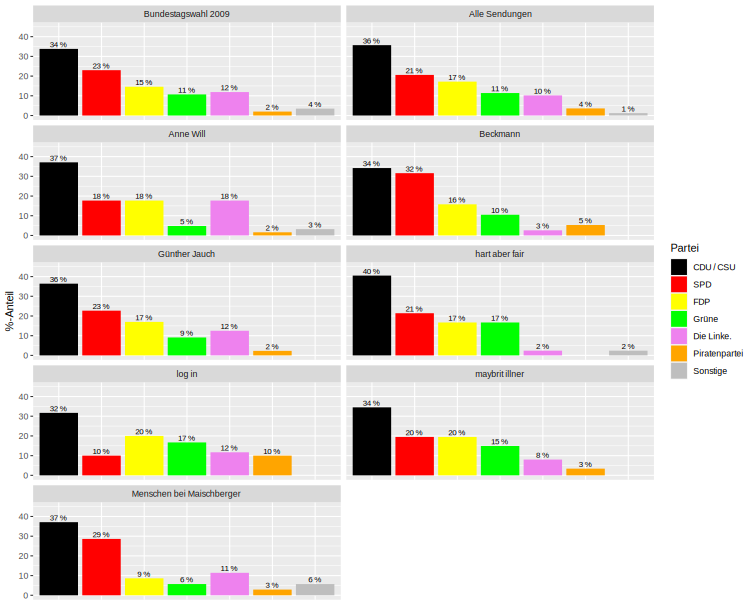
\includegraphics[width=1\textwidth]{daten/grafiken/plot_parteizugehoerigkeit.png}
	%Captions and Labels can be used since this is a figure environment
	\caption{Vergleich Parteienzugehörigkeit mit Bundestagswahl}
	\subcaption*{(vgl. auch ausführliche Tabelle \vref{tab:anhang_parteizugehoerigkeit_sendungen} im Anhang)}
	\label{plot:parteizugehoerigkeit}
\end{figure}

Dennoch zeigen sich bei einigen Sendungen bemerkenswerte Abweichungen. Die CDU / CSU ist in allen Sendungen außer \textit{log in} überrepräsentiert, wenn auch meist in einem relativ kleinen Rahmen. Einzig bei \textit{hart aber fair} beträgt die Abweichung +6,7 \% gegenüber ihrem Ergebnis bei der Bundestagswahl.

Ebenfalls meist häufiger eingeladen waren FDP-Vetreter. Hier liegt die Abweichung zwar auch bis auf zwei Fälle unter fünf Prozent, dennoch ist dies insofern erstaunlich, als die FDP im Untersuchungszeitraum in Umfragen fast konstant unter 5 \% lag, also weit unter ihrem Ergebnis von 2009 (14,6 \%) und zudem bei drei Landtagswahlen nicht wieder in die jeweiligen Parlamente gewählt wurde. Die beiden größten Abweichungen hinsichtlich der FDP gibt es bei \textit{Maischberger}, wo sie 8,6 \% der Politikerauftritte mit ihren Vertreter besetzen konnten und log in, wo sie wiederum auf fast 20 \% kamen. Da wir nicht in die Abläufe der Redaktionen hineinblicken können, kann es sowohl sein, dass die FDP bei beiden Sendungen bewusst seltener bzw. häufiger eingeladen wurde als auch, dass FDP-Politiker sich bewusst gegen bzw. für die Teilnahme in den beiden Formaten entschieden haben. Nichtsdestotrotz handelt es sich dabei um eine  Verletzung des Ausgewogenheitsgebots.

SPD-Politiker sind hingegen bei \textit{Beckmann} relativ häufiger zu Gast (+8,6 \% im Vergleich zu ihrem Bundestagsergebnis), worunter wiederum die Präsenz der Linkspartei leidet (-9,3 \%).

\begin{table}[ht]
	\centering
	\resizebox{\textwidth}{!}{%
		\begin{tabular}{@{}cccccccc@{}}
			\toprule
			\textbf{} & \textbf{CDU / CSU} & \textbf{FDP} & \textbf{SPD} & \textbf{Grüne} & \textbf{Linkspartei} & \textbf{Piratenpartei} & \textbf{Sonstige} \\ \midrule
			\textbf{Anne Will }     & 3,30 \%          & 3,10 \%           & \textbf{-5,30 \%}  & \textbf{-5,90 \%} & \textbf{5,80 \%}  & -0,40 \%         & -0,30 \% \\
			\textbf{Beckmann}       & 0,40 \%          & 1,20 \%           & \textbf{8,60 \%}   & -0,20 \%          & \textbf{-9,30 \%} & 3,30 \%          & -3,50 \% \\
			\textbf{Günther Jauch}   & 2,60 \%   & 2,40 \% & -0,30 \% & -1,60 \% & 0,60 \%     & 0,30 \%       & -3,50 \% \\
			\textbf{hart aber fair} & \textbf{6,70 \%} & 2,10 \%           & -1,60 \%           & \textbf{6,00 \%}  & \textbf{-9,50 \%} & -2,00 \%         & -1,10 \% \\
			\textbf{Maischberger}   & 3,30 \%          & \textbf{-6,00 \%} & \textbf{5,60 \%}   & \textbf{-5,00 \%} & -0,50 \%          & 0,90 \%          & 1,70 \%  \\
			\textbf{log in}         & -2,10 \%         & \textbf{5,40 \%}  & \textbf{-13,00 \%} & \textbf{6,00 \%}  & -0,20 \%          & \textbf{8,00 \%} & -3,50 \% \\
			\textbf{maybrit illner}  & 0,70 \%   & 4,90 \% & -3,50 \% & 4,20 \%  & -3,90 \%    & 1,40 \%       & -3,50 \% \\ \midrule
			\textbf{ARD-Talkschiene} & 3,20 \%   & 1,20 \% & 0,30 \%  & -1,60 \% & -1,30 \%    & 0,30 \%       & -2,10 \% \\
			\textbf{Alle Sendungen}  & 1,90 \%   & 2,60 \% & -2,40 \% & 0,70 \%  & -1,70 \%    & 1,60 \%       & -2,30 \% \\ \bottomrule
		\end{tabular}%
	}
	\caption{Parteizugehörigkeit im Vergleich zum Bundestagswahlergebnis 2009}
	\subcaption*{Abweichungen über 5\% sind hervorgehoben}
	\label{tab:parteizugehoerigkeit}
\end{table}

Wenn nicht zwischen den einzelnen Parteien differenziert wird, sondern zwischen Bundesregierung und Opposition, dann verdeutlicht Abbildung \vref{plot:parteizugehoerigkeit}, dass die Regierungsparteien in fast allen Sendungen, bis auf \textit{Beckmann} und \textit{Maischberger}, im Vergleich zur Opposition überrepräsentiert sind. Besonders deutlich ist dies bei \textit{hart aber fair}, wo CDU/CSU und FDP zusammen auf gut 57 \% aller Politikerauftritte kommen, dort ist zudem die Linkspartei deutlich unterrepräsentiert – faktisch kommt sie kaum vor, genauso wie die Piratenpartei. Damit wird die Beobachtung bestätigt, dass die Regierungsparteien medial überproportional oft vorkommen \parencites{amendtSchwarzgelberKanalDeutsche2012}[144]{hoffmannPolitischeFernsehinterviewsEmpirische1982}.

Beachtenswert ist zudem, dass im Grunde nur die etablierten Parteien eingeladen werden. Neben der großen Ausnahme Piratenpartei, die aufgrund ihrer damaligen Wahlerfolge schlechterdings nicht vollständig ignoriert werden konnte, kommen bloß zwei Vertreter der Freien Wähler und zweimal Jutta Ditfurth von der Kleinstpartei Ökologische Linke vor. Der Ausschluss sowohl links- als auch rechtsradikaler Parteien und Gruppierungen funktioniert hier also weiterhin.

\subsubsection{Sendungen zum Thema Eurokrise}

Ein wenig anders sieht die Verteilung allerdings bei den Sendungen zur Eurokrise aus. Wie aus Abbildung \vref{plot:parteizugehoerigkeit_euro} ersichtlich, kann man zwei Gruppen bilden. Auf der einen Seite die Sendungen in denen CDU / CSU und FDP überrepräsentiert sind und auf der der anderen diejenigen in denen Oppositionsparteien überrepräsentiert sind.

\begin{figure}[ht]
	%Do not try to scale figure in .tex or you loose font size consistency
	\centering
	%The code to input the plot is extremely simple
	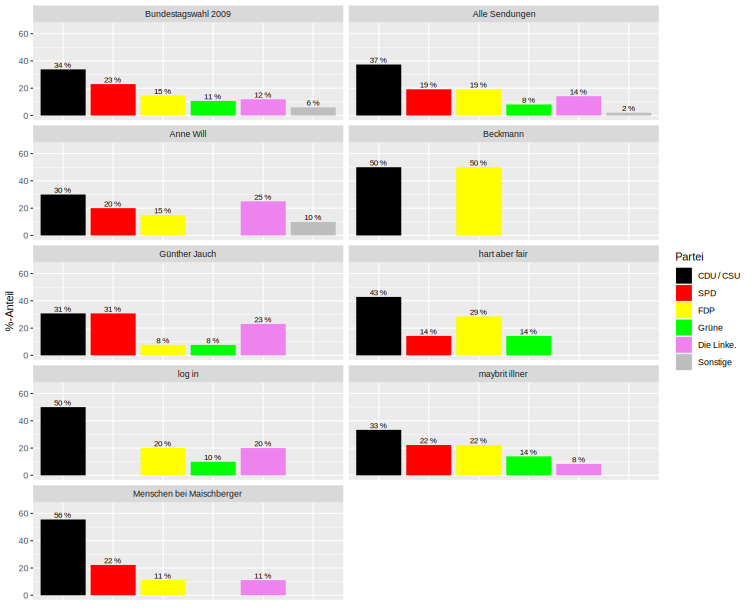
\includegraphics[width=1\textwidth]{daten/grafiken/plot_parteizugehoerigkeit_euro.png}
	%Captions and Labels can be used since this is a figure environment
	\caption{Vergleich Parteienzugehörigkeit mit Bundestagswahl (Sendungen zum Thema Eurokrise)}
	\label{plot:parteizugehoerigkeit_euro}
\end{figure}

Zur ersten Gruppe gehören \textit{Beckmann}, \textit{hart aber fair}, \textit{Menschen bei Maischberger}, \textit{log in} und \textit{maybrit illner}. Besonders eklatant sind die Werte bei \textit{Beckmann}, wo nur Politiker der Regierungsparteien eingeladen waren. Dem gegenüber stehen bloß zwei Sendungen, in denen die Oppositionsparteien häufiger vertreten sind als die Regierungsparteien – \textit{Anne Will} und \textit{Günther Jauch}. Der Regierung fällt es damit wesentlich leichter ihre Positionen zur Eurokrise in den Sendungen unterzubringen als der Opposition.

Parteispezifisch sind zudem die relativ hohen Werte der Linkspartei bei \textit{Anne Will}, \textit{Günther Jauch} und \textit{log in} erwähnenswert. Dafür fehlt die Partei bei \textit{hart aber fair} komplett. Nimmt man alle Sendungen zusammen führt dies dazu, dass die Werte fast dem Ergebnis der letzten Bundestagswahl entsprechen, was auch zeigt, dass gerade die kleineren Parteien vornehmlich zu ihren „Spezialthemen“ eingeladen werden.

\subsection{Demografie}\label{chap:demografie}

Zum Abschluss sollen hier noch die beiden erhobenen demografischen Merkmale – Alter und Geschlecht – näher betrachtet werden.

\subsubsection{Altersstruktur}

Hinsichtlich der Altersstruktur kann bei fast allen Sendungen festgestellt werden, dass das jeweilige Gästepanel im Vergleich zum Bevölkerungsdurchschnitt überaltert ist. Einzig \textit{log in} bewegt sich mit einem Altersdurchschnitt von 45 Jahren relativ nahe am Durchschnittsalter der Bevölkerung von 43,7 Jahren und unterstreicht damit leidlich seine Ausrichtung als „junges“ Format auf ein jüngeres Publikum.

\begin{table}[ht]
	\centering
	\caption{Altersstruktur der Talkshows}
	%\resizebox{\textwidth}{!}{%
		\begin{tabular}{@{}ccccl@{}}
			\toprule
			& \textbf{Median} & \textbf{Min} & \textbf{Max} & \textbf{N}         \\ \midrule
			\textbf{Anne Will}      & 57              & 21           & 92           & 210 (fehlend 4)    \\
			\textbf{Beckmann}       & 51              & 18           & 94           & 156 (fehlend 40)   \\
			\textbf{Günther Jauch} & 57              & 14           & 93           & 189 (fehlend 14)   \\
			\textbf{hart aber fair} & 52              & 18           & 81           & 184 (fehlend 9)    \\
			\textbf{Maischberger}   & 58              & 15           & 94           & 205 (fehlend 33)   \\
			\textbf{log in}         & 45              & 18           & 82           & 143 (fehlend 17)   \\
			\textbf{maybrit illner} & 56              & 20           & 88           & 219 (fehlend 18)   \\ \midrule
			\textbf{ARD-Talks}      & 56              & 14           & 94           & 1087 (fehlend 100) \\
			\textbf{Alle Sendungen} & 54              & 14           & 94           & 1306 (fehlend 134) \\ \bottomrule
		\end{tabular}%
	%}
	\label{tab:altersstruktur}
\end{table}

Die „älteste“ Sendung ist \textit{Menschen bei Maischberger}, wo die Gäste im Schnitt fast 58 Jahre alt sind, dicht gefolgt von\textit{ Günther Jauch} mit circa 56 Jahren. Der „jüngste“ ARD-Polittalk ist hart aber fair mit einem Durchschnitt von knapp 53 Jahren. Insgesamt sind die Unterschiede zwischen den sechs etablierten Talks aber vernachlässigbar (vgl. Tabelle \vref{tab:altersstruktur}).

Die Problematik dieser Überalterung zeigt sich noch deutlicher, wenn man sich vor Augen führt, dass nur 3,7 \% der Gäste unter 30 Jahre alt waren, während die Altersgruppe der 40 bis 69jährigen 61,5 \% der Gäste und selbst die über 80jährigen noch 4,5 \% ausmachten. Die jüngeren Generationen selbst – und damit wahrscheinlich auch ihre politischen Meinungen und Ansichten – kommen folglich kaum vor in den Sendungen.

Da das Phänomen in sechs der sieben Talks auftritt, kann es auch nur bedingt über eine bestimmte Zielgruppenausrichtung erklärt werden. Zwar könnte man durchaus den hohen Altersschnitt bei \textit{Menschen bei Maischberger} mit einer gezielten Ansprache eines ebenfalls älteren Publikums erklären – und rechtfertigen. Die gleiche Begründung kann aber etwa bei \textit{Günther Jauch} oder \textit{maybrit illner} nicht angewendet werden, richten sich diese Sendungen doch ihrem Anspruch nach an die gesamte Bevölkerung.

Allerdings kann die Altersstruktur vielleicht erklären, warum die Konsumenten von Polittalks, zumindest vor zehn Jahren, mit einem Schnitt von 62 bis 64 Jahren ein noch höheres Alter aufwiesen \parencite[309f.]{gerhardsTalkshownutzungUndTalkshownutzer2002}.

\subsubsection{Geschlechterverhältnis}

Ein ähnlich ernüchterndes Bild wie bei der Altersstruktur ergibt ein Blick auf das Geschlechterverhältnis der eingeladenen Gäste.

\begin{figure}[ht]
	%Do not try to scale figure in .tex or you loose font size consistency
	\centering
	%The code to input the plot is extremely simple
	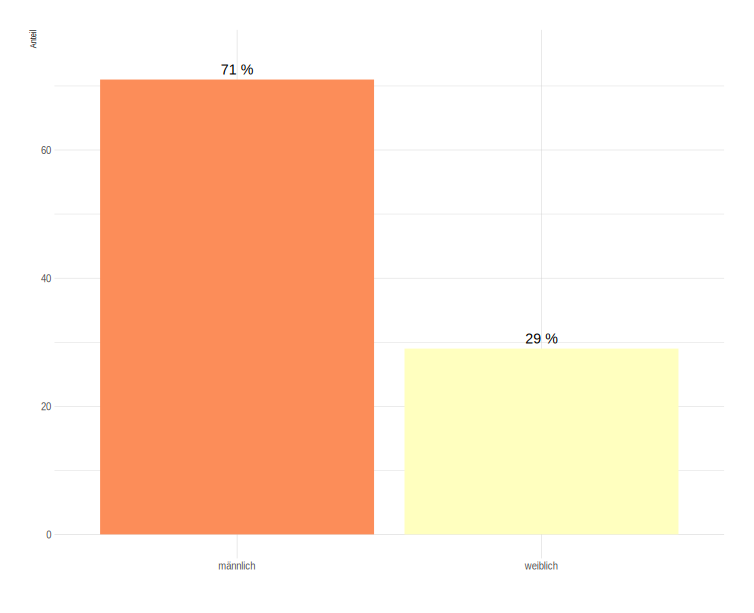
\includegraphics[width=1\textwidth]{daten/grafiken/plot_geschlechterverhaeltnis_gesamt.png}
	%Captions and Labels can be used since this is a figure environment
	\caption{Geschlechterverhältnis der Gäste}
	\subcaption*{alle Sendungen; n = 1441}
	\label{plot:geschlechterverhaeltnis_gesamt}
\end{figure}

Wie aus der obigen Abbildung ersichtlich wird, dominieren unter den Gästen Männer mit über 70 \%. Hält man sich vor Augen, dass in Deutschland das Verhältnis zwischen Männern und Frauen bei 51 \% zu 49 \% liegt \parencite{statistischesbundesamtBevoelkerungsstand2011}, so wird klar, dass die untersuchten Sendungen hier eklatant gesellschaftliche Ungleichheit reproduzieren\footnote{Solche Ungleichheiten zeigen sich etwa in der weiterhin schlechteren Bezahlung von Frauen oder dem ungleichen Zugang zu Führungspositionen in Politik und Wirtschaft \parencite{hausmannGlobalGenderGap2012}}.

Die Tendenz ist dabei bei alle Talksendungen gleich (vgl. Abbildung \vref{plot:geschlechterverhaeltnis_sendungen}), auffallend sind einzig die beiden ZDF-Talks, da bei ihnen das Verhältnis noch ungünstiger ist, und die beiden „weicheren“ ARD-Formate \textit{Beckmann} und \textit{Menschen bei Maischberger}, bei denen das Verhältnis ein wenig ausgeglichener ist.

\begin{figure}[ht]
	%Do not try to scale figure in .tex or you loose font size consistency
	\centering
	%The code to input the plot is extremely simple
	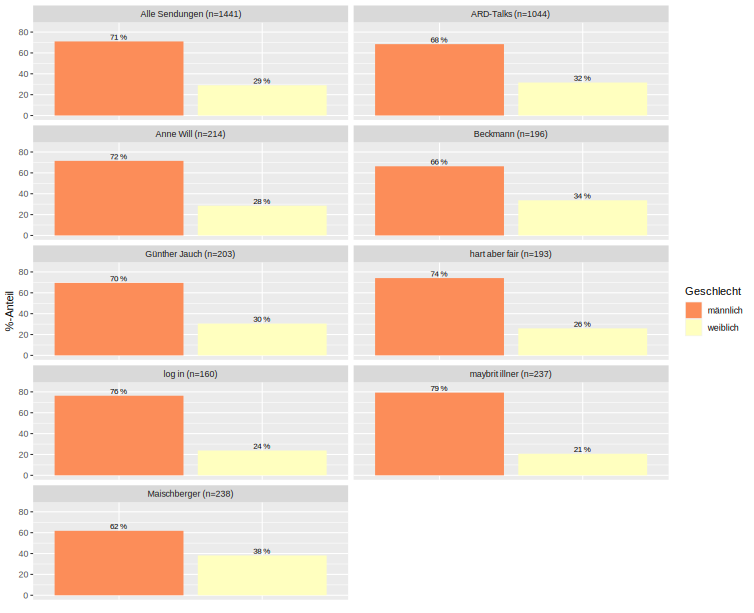
\includegraphics[width=1\textwidth]{daten/grafiken/plot_geschlechterverhaeltnis_sendungen.png}
	%Captions and Labels can be used since this is a figure environment
	\caption{Geschlechterverhältnis der Gäste nach Sendungen}
	\label{plot:geschlechterverhaeltnis_sendungen}
\end{figure}

Wird das Geschlechterverhältnis nach Themenbereichen aufgeschlüsselt, so kann man feststellen, dass in Sendungen zu Kriminalität und Katastrophen, zu Prominenz oder Gesundheit sowie bei sonstigen Themen, der Anteil weiblicher Gäste deutlich größer ist als bei Themen aus den Bereichen Politik, Wirtschaft oder auch Sport (vgl. Abbildung \vref{plot:geschlechterverhaeltnis_themen}).

\begin{figure}[ht]
	%Do not try to scale figure in .tex or you loose font size consistency
	\centering
	%The code to input the plot is extremely simple
	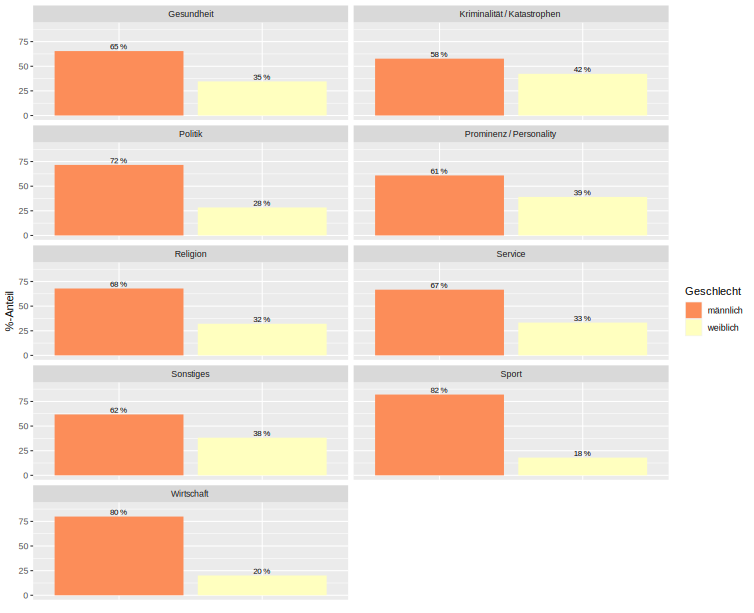
\includegraphics[width=1\textwidth]{daten/grafiken/plot_geschlechterverhaeltnis_themen.png}
	%Captions and Labels can be used since this is a figure environment
	\caption{Geschlechterverhältnis der Gäste nach Themenbereichen}
	\label{plot:geschlechterverhaeltnis_themen}
\end{figure}

Es scheint also so, als ob die Redaktionen bei unpolitischeren, boulevardesken Themen eher Frauen einladen als bei den seriösen Themen. Damit reproduzieren die Sendungen gesellschaftliche Ungleichheiten. So liegt der Frauenanteil im Bundestag beispielsweise  nur bei knapp 33 \% (Deutscher Bundestag 2011) und Führungspositionen in der Wirtschaft werden ebenfalls nur zu 30 \% von Frauen besetzt \parencite{hostFuhrungskrafteMonitor20122012}.

Wenn man bedenkt, dass Medien nicht bloß die Realität widerspiegeln, sondern sie mit schaffen und beeinflussen, ist es nicht einzusehen, warum politische Talkshows existierende soziale Ungleichheiten bloß reproduzieren, anstatt versuchen diese auszugleichen. Zumal die öffentlich-rechtlichen Sender in den entsprechenden Gesetzen zur Förderung der Gleichstellung verpflichtet sind (vgl. Kapitel \vref{chap:anforderungen}). Zumal sich hier ein Zustand vorsetzt, der bereits an \textit{Sabine Christiansen} kritisiert wurde, deren Frauenanteil allerdings noch bei nur 12 \% lag \parencite[3]{muellerSchaubuehneFuerEinflussreichen2006}.

\section{Zwischenfazit}

Die Untersuchung der Themenstruktur ergab, dass sich die Sendung anhand der abgedeckten Themenbereiche in zwei Gruppen einteilen lassen. Zum einen die reinen Polittalks, die sich überwiegend mit rein politischen Themen befassen und zum anderen die in Richtung Personality-Show tendierenden Formate, die einen bunteren Themenmix bieten der auch unpolitische Themen enthält. Zur ersten Gruppe gehören \textit{Anne Will}, \textit{Günther Jauch}, \textit{log in} und \textit{maybrit illner}, zur zweiten Beckmann, \textit{Menschen bei Maischberger} und – erstaunlicherweise – \textit{hart aber fair}.

Unter den politischen Themen dominiert bei allen Sendungen die Innenpolitik klar. Daneben spielen nur noch sozialpolitische Themen eine nennenswerte Rolle. Alle erfassten Politikbereiche kommen einzig bei \textit{Günther Jauch} vor. log in kennzeichnet ein relativ hoher Anteil umweltpolitischer Thematiken.

Doppelungen, bei denen verschiedene Sendungen das gleiche Thema in kurzer Zeit behandeln, lassen sich immer wieder finden. Insbesondere bei aktuellen „Aufregerthemen“ wie der Wulff-Affäre ist dies der Fall, aber auch bei zeitlosen Thematiken wie dem Burnout-Syndrom. Hinzukommt, dass sich die Titel vieler Talkfolgen durch einen alarmistischen Grundton und einseitige Vorfestlegungen statt neutraler Formulierungen auszeichnen.

Resümierend lässt sich festhalten, dass der ARD-Programmausschuss mit folgender Ein"-schätz"-ung der hauseigenen Talkschiene weitgehend richtig liegt:

\begin{quote}
	„Alle-fünf (sic!) Talk-Sendungen sind unpolitischer geworden, was dazu führt, dass wichtige, gesellschaftlich relevante Themen, die komplex und somit er"-klärungs"-be"-dürf"-tig sind, nicht behandelt werden. Nach wie vor fehlen wirtschaftspolitische Themen sowie unterschiedliche Themen der Sozial- und Energiepolitik fast völlig, ebenso wie neue politische Bewegungen und die Internationale Politik. Auch die Wirtschafts- und Finanzmarktkrise in Europa wird nicht adäquat und genügend differenziert behandelt, Hinzu (sic!) kommt, dass es nach wie vor Themendoppelungen gibt (z. B. Essen, Gesundheit), dio (sic!) nicht notwendig sind.“ \parencite{harbuschGeheimPapierARDKritisiert2012}
\end{quote}

Allerdings kann man diese Diagnose aufgrund der hier vorliegenden Daten zugleich einschränken als auch erweitern. Von einer Häufung unpolitischer Themen kann im Grunde nur bei hart aber fair gesprochen werden. Sowohl \textit{Anne Will} als auch \textit{Günther Jauch} haben einen hohen Anteil an politischen Themen im engeren Sinne und \textit{Beckmann} bzw. \textit{Menschen bei Maischberger} dürften aufgrund ihrer Nähe zu Personality-Talks bereits mehr unpolitische Themen geboten haben. Auch ob die Finanz- und Eurokrise nicht ausreichend berücksichtigt wurde, ist zumindest Interpretationssache, wurde das Thema doch innerhalb eines Jahres immerhin 24-mal von den ARD-Talks behandelt (vgl. Tabelle \vref{tab:themencluster}) – ob sie hingegen differenziert genug behandelt wurde, wird die folgende qualitative Sendungsanalyse zeigen. Auszuweiten ist die Diagnose hingegen insofern, als dass sie nicht nur auf die ARD-Talkschiene zutrifft, sondern ebenso auf die beiden untersuchten Polittalks des ZDF – auch bei diesen werden viele politische Themenfelder vernachlässigt und es kommt zu Themendoppelungen mit den anderen öffentlich-rechtlichen Talks. Diese Einseitigkeiten schränken sowohl Pluralität als auch Relevanz der Sendungen ein.

Hinsichtlich der Gästestruktur lässt sich resümieren, dass der Anteil von Politikern je nach Thema und Sendung relativ hoch ist. Dies gilt vor allem für die jeweiligen Talkflaggschiffe \textit{Günther Jauch} und \textit{maybrit illner}. Gleichzeitig ist die Dominanz allerdings nicht mehr ganz so stark ausgeprägt wie noch 1999, als über zwei Drittel der Gäste bei \textit{Sabine Christiansen} Politiker waren \parencite[141]{doernerPolitainmentPolitikMedialen2001}.

Allerdings zeichnet sich die Gruppe der Politiker durch eine hohe Zahl an mehreren Auftritten der gleichen Personen aus. Dies ist bei den anderen Gästegruppen im Allgemeinen nicht in derartigem Ausmaß der Fall, somit kann von einer talkenden Politikerelite gesprochen werden. Speziell beim Thema Eurokrise lässt sich allerdings ein Absinken des Wiederholungsquotienten bei Politiker und ein Anstieg bei Experten und Wirtschaftsvertretern feststellen. Hier ist also eher von einer Elite von Personen aus den drei Gruppen zu sprechen.

Die Gruppe der Politiker zeichnet sich darüber hinaus durch ein Übergewicht von Bundespolitikern aus. Bei der Parteizugehörigkeit zeigt sich hingegen der Versuch den Proporz zu wahren. Dies gelingt mehr oder weniger gut, allerdings gibt es bei sechs der sieben Sendungen eine Übervorteilung der Regierungsparteien im Vergleich zum Ergebnis der letzten Bundestagswahl. Am größten ist diese Verzerrung bei \textit{hart aber fair}. \textit{log in} sticht hingegen durch eine häufige Einladung von Vertretern der Piratenpartei hervor. Bei den Talks, welche die Eurokrise behandeln, ist die Überrepräsentation der Regierungsparteien nochmals um ein gutes Stück größer. Hier ist \textit{Beckmann} der Extremfall, wo keinerlei Oppositionspolitiker zu Wort kommen. Die Verzerrung bei \textit{maybrit illner} ist allerdings aufgrund der höheren Anzahl an politischen Gästen und Folgen zur Eurokrise aufs Ganze betrachtet problematischer.

Im Bereich der Wirtschaftsvertreter zeigt sich eine eklatante Verzerrung zu Gunsten von wirtschaftsnahen Personen, die bei den Folgen zur Eurokrise nochmals stärker ist. Ähnliches gilt für Vertreter der Zivilgesellschaft, die nur in geringem Umfang in den Sendungen zu Wort kamen – mit Ausnahme von \textit{log in} – und damit nicht die Dominanz der Wirtschaft ausgleichen können, zumal die klassischen Sozialverbände nur noch selten eingeladen werden. Hiermit setzt sich eine Diagnose fort, die bereits in gleicher Weise für \textit{Sabine Christiansen} galt \parencite[7]{muellerSchaubuehneFuerEinflussreichen2006}. Bei Journalisten und Experten gibt es keine ungewöhnlichen Auffälligkeiten. \textit{Beckmann} und \textit{Menschen bei Maischberger} setzten entsprechend ihrer thematischen Ausrichtung stark auf Ärzt, \textit{hart aber fair} auf sonstige Experten und die restlichen Talks auf Wissenschaftler.

Ebenfalls große Abweichungen zeigen die beiden demografischen Indikatoren. Sowohl was das Alter der Gäste als auch ihr Geschlecht an geht, weichen die Sendungen stark vom gesellschaftlichen Durchschnitt ab. Das Format mit den jüngsten Gästen ist wenig überraschend log in. Beim Geschlechterverhältnis sind \textit{Beckmann} und \textit{Menschen bei Maischberger} am nächsten an der realen Verteilung, allerdings nur weil zu unpolitischen Themen tendenziell mehr Frauen eingeladen werden als zu politischen.

Die Talkshows insgesamt reproduzieren also gesellschaftliche Ungleichheiten – sei es die Benachteiligung von Frauen, die Überalterung politischer Debatten, die größere mediale Präsenz der Regierungsparteien oder die Dominanz arbeitgebernaher Positionen. Zudem verstoßen sie durch eine teils einseitige und doppelte Themenwahl sowie die hohe Gästewiederholung bei Politikern ebenfalls gegen die geforderte Pluralität, Ausgewogenheit und Relevanz.